% Capstone Project Phase-1 report: AI-Driven Analysis and Optimization of CI/CD
% Pipelines for Build Failure Prediction.  Build: latexmk -pdf main.tex
\documentclass[12pt,a4paper,oneside]{report}

% ---- Page, font and spacing: VI-semester capstone report guidelines ----
\usepackage[a4paper,top=2.5cm,bottom=2.5cm,left=2.75cm,right=2.25cm]{geometry}
\usepackage[T1]{fontenc}
\usepackage{newtxtext,newtxmath}          % Times New Roman
\usepackage{setspace}\onehalfspacing      % line spacing 1.5
\usepackage[parfill]{parskip}             % paragraphs separated by space, as in the draft
\usepackage{microtype}
\usepackage{ragged2e}

\usepackage{graphicx,xcolor,array,longtable,booktabs,multirow,tabularx,makecell}
\usepackage{amsmath}
\usepackage{enumitem}
\usepackage{tikz}
\usetikzlibrary{arrows.meta,positioning,shapes.geometric,shapes.multipart,fit,calc,backgrounds}
\usepackage{caption}
\usepackage{float}
\usepackage{chngcntr}
\usepackage[hidelinks]{hyperref}
\usepackage{url}
\urlstyle{same}

\graphicspath{{images/}{figures/}{../paper/figures/}{../paper/screens/}}

% ---- Headings: chapter 14 pt all caps, sections 14 pt bold, subsections 12 pt bold ----
\usepackage{titlesec}
\titleformat{\chapter}[hang]{\fontsize{14}{17}\selectfont\bfseries}{CHAPTER \thechapter\ --}{0.4em}{\MakeUppercase}
\titlespacing*{\chapter}{0pt}{0pt}{16pt}
\titleformat{\section}{\fontsize{14}{17}\selectfont\bfseries}{\thesection}{0.6em}{}
\titleformat{\subsection}{\fontsize{12}{15}\selectfont\bfseries}{\thesubsection}{0.6em}{}
\titlespacing*{\section}{0pt}{14pt}{6pt}
\titlespacing*{\subsection}{0pt}{10pt}{4pt}
\newcommand{\minorhead}[1]{\par\vspace{4pt}\noindent\textbf{#1}\par}

% ---- Captions: "Fig N:" numbered through the report; tables numbered per chapter ----
\counterwithout{figure}{chapter}
\captionsetup{font=small,labelfont=bf,labelsep=colon,justification=centering}
\captionsetup[figure]{name=Fig}
\captionsetup[table]{name=Table,position=top}
\setlength{\abovecaptionskip}{6pt}

\setlist{itemsep=2pt,topsep=4pt}
\renewcommand{\arraystretch}{1.25}
\newcolumntype{L}{>{\RaggedRight\arraybackslash}X}
\newcommand{\tierC}{Tier~C}
\newcommand{\tierE}{Tier~E}
\newcommand{\dAUC}{$\Delta$AUC}
\definecolor{vtured}{RGB}{204,0,0}
\definecolor{titlegreen}{RGB}{56,118,29}
\definecolor{deptblue}{RGB}{17,85,204}
\definecolor{sigblue}{RGB}{61,133,198}

\AtBeginDocument{\justifying}

\begin{document}
% ---------------------------------------------------------------- Title page
\begin{titlepage}
\centering
\singlespacing
\setlength{\parskip}{3pt}
{\fontsize{16}{20}\selectfont\bfseries\color{vtured} VISVESVARAYA TECHNOLOGICAL UNIVERSITY\par}
\vspace{2pt}
{\large Jnana Sangama, Belagavi - 590 018, Karnataka\par}
\vspace{6pt}

\includegraphics[width=2.0cm]{vtu_logo.png}\par
\vspace{8pt}
{\large\bfseries Capstone Project Phase -- 1\par (Course code: 24AM6PWPW1)\par}
\vspace{8pt}
{\large\bfseries PROJECT WORK REPORT\par}
\vspace{10pt}
{\fontsize{18}{24}\selectfont\bfseries\color{titlegreen} AI-Driven Analysis and Optimization of CI/CD\\[2pt] Pipelines for Build Failure Prediction\par}
\vspace{10pt}
{\large\itshape In the Department of\par}
{\Large\bfseries\color{deptblue} Machine Learning\par}
{\large\bfseries (UG Program: B.E. in Artificial Intelligence and Machine Learning)\par}
{\large Submitted by\par}
\vspace{6pt}
{\bfseries
\begin{tabular}{@{}l@{\hspace{1.2em}}l@{}}
\textcolor{deptblue}{Pakam Yasaswini} & \textcolor{titlegreen!70!black}{1BM23AI121}\\
\textcolor{deptblue}{Reem Rashid} & \textcolor{titlegreen!70!black}{1BM23AI148}\\
\textcolor{deptblue}{Sarayu KS} & \textcolor{titlegreen!70!black}{1BM23AI171}
\end{tabular}\par}
\vspace{4pt}
{\color{titlegreen!70!black} 6th Semester\par}
\vspace{6pt}
{\large Under the Guidance of\par}
\vspace{4pt}
{\large\bfseries\color{deptblue} Dr. Rajeshwari M.R.\par}
\vspace{3pt}
Designation\par
Dept. of MEL, BMSCE, Bengaluru -- 19\par
\vspace{8pt}

\includegraphics[width=2.1cm]{bmsce_logo.png}\par
\vspace{8pt}
{\Large\bfseries\color{deptblue} DEPARTMENT OF MACHINE LEARNING\par}
\vspace{4pt}
{\fontsize{18}{22}\selectfont\bfseries\color{vtured} B.M.S. COLLEGE OF ENGINEERING\par}
{\small\itshape (An Autonomous Institute, Affiliated to VTU)\par}
P.O. Box No. 1908, Bull Temple Road, Bengaluru - 560 019\par
\end{titlepage}

% ---------------------------------------------------------------- Certificate
\thispagestyle{empty}
\begin{center}
\singlespacing
{\fontsize{16}{20}\selectfont\bfseries\color{vtured} B.M.S COLLEGE OF ENGINEERING\par}
{\small (An Autonomous Institute, Affiliated to VTU)\par}
P.O. Box No. 1908, Bull Temple Road, Bengaluru - 560 019\par
\vspace{14pt}
{\Large\bfseries\color{deptblue} DEPARTMENT OF MACHINE LEARNING\par}
\vspace{12pt}

\includegraphics[width=2.4cm]{bmsce_logo.png}\par
\vspace{12pt}
{\large\bfseries CERTIFICATE\par}
\end{center}
\vspace{6pt}
This is to certify that \textcolor{deptblue}{Ms.\ Pakam Yasaswini} bearing \textcolor{deptblue}{USN: 1BM23AI121}, \textcolor{deptblue}{Ms.\ Reem Rashid} bearing \textcolor{deptblue}{USN: 1BM23AI148}, and \textcolor{deptblue}{Ms.\ Sarayu K S} bearing \textcolor{deptblue}{USN: 1BM23AI171} have satisfactorily completed the Course -- Capstone Project Work (Course Code: 24AM6PWPW1) with the title \textcolor{deptblue}{\textbf{``AI-Driven Analysis and Optimization of CI/CD Pipelines for Build Failure Prediction''}} in partial fulfillment of academic curriculum requirements of the 6th semester UG Program -- B.\,E. in Artificial Intelligence and Machine Learning in the Department of Machine Learning, BMSCE, an Autonomous Institute, affiliated to Visvesvaraya Technological University, Belagavi during May 2026. It is also stated that the base work considered for the presentation is used only for academic purpose and not used in its original form anywhere for award of any degree.

\vspace{10pt}
\textbf{Student Signature}

\vspace{30pt}
\noindent\begin{tabular}{@{}p{0.5\textwidth}p{0.45\textwidth}@{}}
\textbf{Signature of the Faculty,} & \textbf{Signature of the Head}\\[12pt]
\textcolor{sigblue}{\textbf{Dr. Rajeshwari M.R.}} & \textbf{Dr. M Dakshayini}\\
Designation, Dept. of MEL, BMSCE & Prof. \& Head, Dept. of MEL, BMSCE
\end{tabular}

\vspace{24pt}
\begin{center}\large\bfseries External Examination\end{center}
\hspace{1em}\textbf{Examiner Name and Signature}

\textbf{1.}

\textbf{2.}
\clearpage

% ---------------------------------------------------------------- Declaration
\pagenumbering{roman}
\setcounter{page}{1}
\begin{center}\fontsize{14}{17}\selectfont\bfseries DECLARATION\end{center}
\label{fm:declaration}
We, Ms.\ Pakam Yasaswini bearing USN: 1BM23AI121, Ms.\ Reem Rashid bearing USN: 1BM23AI148, and Ms.\ Sarayu K S bearing USN: 1BM23AI171, hereby declare that the project titled ``AI-Driven Analysis and Optimization of CI/CD Pipelines for Build Failure Prediction'' is an original work carried out by us under the guidance of Dr.\ Rajeshwari M.R., Assistant Professor, at BMSCE, Bengaluru. The work presented in this report has not been submitted elsewhere for any other degree, diploma, or certification.

We declare that all the references and sources used in the report have been properly acknowledged and cited. No part of this report has been copied, plagiarized, or reproduced from another work without proper attribution.

\vspace{30pt}
\begin{flushright}
\begin{tabular}{@{}l@{}}
Pakam Yasaswini -- (USN: 1BM23AI121)\\
Reem Rashid -- (USN: 1BM23AI148)\\
Sarayu KS -- (USN: 1BM23AI171)
\end{tabular}
\end{flushright}
\clearpage

% ---------------------------------------------------------------- Acknowledgement
\begin{center}\fontsize{14}{17}\selectfont\bfseries ACKNOWLEDGEMENT\end{center}
\label{fm:ack}
We would like to express our deepest gratitude and sincere thanks to our guide Dr.\ Rajeshwari M.R., Assistant Professor, Department of Machine Learning, BMSCE, Bengaluru, for her keen interest, continuous guidance, and encouragement in bringing this project work to completion.

We are grateful to Dr.\ M.\ Dakshayini, Professor and Head, Department of Machine Learning, Bengaluru, for her valuable suggestions and support throughout the project work.

We express our profound gratitude to the Hon'ble Management and Dr.\ Bheemsha Arya, Principal, BMSCE, Bengaluru, for providing the necessary facilities and a supportive environment to carry out this project successfully.

We would also like to thank all the staff members of the Department of Machine Learning for their support, encouragement, and guidance during the course of this project.

Last but not the least, we would like to thank our parents, family, and friends whose constant encouragement and support made this work possible.

\vspace{30pt}
\begin{flushright}
\begin{tabular}{@{}l@{}}
Pakam Yasaswini -- (USN: 1BM23AI121)\\
Reem Rashid -- (USN: 1BM23AI148)\\
Sarayu KS -- (USN: 1BM23AI171)
\end{tabular}
\end{flushright}
\clearpage

% ---------------------------------------------------------------- Abstract
\begin{center}\fontsize{14}{17}\selectfont\bfseries ABSTRACT\end{center}
\label{fm:abstract}
Continuous integration and continuous deployment (CI/CD) pipelines are central to modern software development, but failed builds still interrupt developers, delay releases and waste compute. CI/CD platforms automate and monitor pipelines; they offer little help in predicting which builds will fail, diagnosing why, or spotting slow stages.

This project builds and evaluates an AI-driven system that predicts build failures \emph{before} a build runs, detects slow or stalled pipeline jobs, groups failure logs to suggest root causes, and presents the results on an interactive dashboard. The predictor was developed on 858,368 Travis~CI builds from 947 open-source projects and evaluated on 146,556 GitHub Actions runs from 60 further projects.

A central finding is that the usual way of measuring these models greatly overstates them. With a random train/test split, classifiers such as Random Forest, Decision Tree and SVM appear strong (AUC up to 0.91), but they quietly use future information. Under a strict protocol, the same task scores 0.63. That protocol uses only information available when a build is triggered, counts a past build only once it has finished, evaluates chronologically, and measures how well a model ranks \emph{each repository's own} builds. Within this protocol, our final model (\tierE) adds the history of the build's own branch or pull request, the state of builds still running, and a learning-to-rank objective. It improves within-repository AUC from 0.628 to 0.698 on Travis~CI, including on builds that break a previously passing branch (0.556 to 0.622).

We then tested the frozen model on GitHub Actions with protocols fixed and hashed before collecting any data. The first test (30 repositories) improved in every fold but was inconclusive under the pre-registered rule. A confirmation on 30 new repositories met the rule in all five folds (0.911 vs.\ 0.763).

The deployed system receives GitHub webhooks and scores each workflow run when it is requested. Each repository's riskiest 15\% of recent runs are flagged as alerts, which catches about 41\% of a repository's failures. A read-only public demonstration and a pre-registered forward-looking test of the frozen system complete the work.

\clearpage

% ---------------------------------------------------------------- Table of contents (bordered, as in the template)
\begin{center}\fontsize{14}{17}\selectfont\bfseries TABLE OF CONTENTS\end{center}
\label{fm:toc}
{\setlength{\extrarowheight}{2pt}\renewcommand{\arraystretch}{1.15}
\begin{longtable}{|>{\centering\arraybackslash}p{1.1cm}|p{11.6cm}|>{\centering\arraybackslash}p{1.4cm}|}
\hline
\multicolumn{2}{|l|}{\textbf{Declaration}} & \textbf{\pageref{fm:declaration}}\\
\multicolumn{2}{|l|}{\textbf{Acknowledgement}} & \textbf{\pageref{fm:ack}}\\
\multicolumn{2}{|l|}{\textbf{Abstract}} & \textbf{\pageref{fm:abstract}}\\
\multicolumn{2}{|l|}{\textbf{Table of Contents}} & \textbf{\pageref{fm:toc}}\\
\multicolumn{2}{|l|}{\textbf{List of Figures}} & \textbf{\pageref{fm:lof}}\\
\multicolumn{2}{|l|}{\textbf{List of Tables}} & \textbf{\pageref{fm:lot}}\\ \hline
\textbf{1} & \textbf{INTRODUCTION} & \textbf{\pageref{ch:intro}}\\ \hline
 & 1.1 Overview & \pageref{sec:overview}\\ \hline
 & 1.2 Summary of the Work Carried Out & \pageref{sec:summarywork}\\ \hline
 & 1.3 Organization of the Report & \pageref{sec:organization}\\ \hline
\textbf{2} & \textbf{PROBLEM STATEMENT} & \textbf{\pageref{ch:problem}}\\ \hline
 & 2.1 Problem Statement & \pageref{sec:problem}\\ \hline
 & 2.2 Motivation & \pageref{sec:motivation}\\ \hline
 & 2.3 Objectives and Scope & \pageref{sec:objectives}\\ \hline
\textbf{3} & \textbf{LITERATURE SURVEY} & \textbf{\pageref{ch:lit}}\\ \hline
 & 3.1 Existing Systems & \pageref{sec:existing}\\ \hline
 & 3.2 Research on Build Failure Prediction & \pageref{sec:research}\\ \hline
 & 3.3 Research Gap & \pageref{sec:gap}\\ \hline
\textbf{4} & \textbf{SYSTEM REQUIREMENT SPECIFICATION} & \textbf{\pageref{ch:srs}}\\ \hline
 & 4.1 Functional Requirements & \pageref{sec:functional}\\ \hline
 & 4.2 Non-functional Requirements & \pageref{sec:nonfunctional}\\ \hline
 & 4.3 Hardware Requirements & \pageref{sec:hardware}\\ \hline
 & 4.4 Software Requirements & \pageref{sec:software}\\ \hline
\textbf{5} & \textbf{SYSTEM DESIGN} & \textbf{\pageref{ch:design}}\\ \hline
 & 5.1 System Architecture & \pageref{sec:architecture}\\ \hline
 & 5.2 Proposed Methodology & \pageref{sec:methodology}\\ \hline
 & 5.3 Detailed Design & \pageref{sec:detailed}\\ \hline
 & \hspace{1.2em}5.3.1 Class Diagram & \pageref{sec:class}\\ \hline
 & \hspace{1.2em}5.3.2 Activity Diagram & \pageref{sec:activity}\\ \hline
 & \hspace{1.2em}5.3.3 Use Case Diagram & \pageref{sec:usecase}\\ \hline
\textbf{6} & \textbf{IDENTIFICATION OF TOOLS AND TECHNIQUES} & \textbf{\pageref{ch:tools}}\\ \hline
 & 6.1 Development Tools & \pageref{sec:devtools}\\ \hline
 & 6.2 CI/CD and Integration Tools & \pageref{sec:citools}\\ \hline
 & 6.3 Visualization and Deployment Tools & \pageref{sec:viztools}\\ \hline
 & 6.4 Techniques Used & \pageref{sec:techniques}\\ \hline
\textbf{7} & \textbf{IMPLEMENTATION} & \textbf{\pageref{ch:impl}}\\ \hline
 & 7.1 Datasets & \pageref{sec:datasets}\\ \hline
 & 7.2 Leakage-Safe Data Pipeline & \pageref{sec:pipeline}\\ \hline
 & 7.3 Feature Engineering & \pageref{sec:features}\\ \hline
 & 7.4 Prediction Models & \pageref{sec:models}\\ \hline
 & 7.5 Anomaly, Bottleneck and Root Cause Modules & \pageref{sec:aux}\\ \hline
 & 7.6 Deployed System & \pageref{sec:deployed}\\ \hline
 & 7.7 Dashboard & \pageref{sec:dashboard}\\ \hline
 & 7.8 Testing and Requirement Traceability & \pageref{sec:testing}\\ \hline
\textbf{8} & \textbf{RESULTS AND DISCUSSION} & \textbf{\pageref{ch:results}}\\ \hline
 & 8.1 Evaluation Protocol & \pageref{sec:protocol}\\ \hline
 & 8.2 How Much the Usual Evaluation Overstates Results & \pageref{sec:leakage}\\ \hline
 & 8.3 Results on Travis CI & \pageref{sec:travis}\\ \hline
 & 8.4 New Breakages & \pageref{sec:newbreak}\\ \hline
 & 8.5 Pre-Registered Tests on GitHub Actions & \pageref{sec:gha}\\ \hline
 & 8.6 Deployed Model and Alert Policy & \pageref{sec:alerts}\\ \hline
 & 8.7 Negative Results & \pageref{sec:negative}\\ \hline
 & 8.8 Threats to Validity & \pageref{sec:threats}\\ \hline
\textbf{9} & \textbf{CONCLUSION AND FUTURE WORK} & \textbf{\pageref{ch:conclusion}}\\ \hline
\textbf{10} & \textbf{REFERENCES} & \textbf{\pageref{ch:references}}\\ \hline
\end{longtable}}
\clearpage

% ---------------------------------------------------------------- List of figures
\begin{center}\fontsize{14}{17}\selectfont\bfseries LIST OF FIGURES\end{center}
\label{fm:lof}
{\renewcommand{\arraystretch}{1.2}
\begin{longtable}{|>{\centering\arraybackslash}p{1.6cm}|p{11.2cm}|>{\centering\arraybackslash}p{1.3cm}|}
\hline
\textbf{Figure No.} & \textbf{Description} & \textbf{Page}\\ \hline
\endhead
Fig \ref{fig:overview} & Overview of the AI-driven CI/CD optimization system & \pageref{fig:overview}\\ \hline
Fig \ref{fig:arch} & System architecture of the proposed CI/CD optimization framework & \pageref{fig:arch}\\ \hline
Fig \ref{fig:method} & Proposed methodology for AI-driven CI/CD pipeline optimization & \pageref{fig:method}\\ \hline
Fig \ref{fig:class} & Class diagram of the CI/CD optimization system & \pageref{fig:class}\\ \hline
Fig \ref{fig:activity} & Activity diagram of the CI/CD optimization system & \pageref{fig:activity}\\ \hline
Fig \ref{fig:usecase} & Use case diagram of the CI/CD optimization system & \pageref{fig:usecase}\\ \hline
Fig \ref{fig:logflow} & Log clustering flow for root cause analysis & \pageref{fig:logflow}\\ \hline
Fig \ref{fig:scoring} & Scoring path of the deployed system & \pageref{fig:scoring}\\ \hline
Fig \ref{fig:dash_overview} & Dashboard: summary cards and daily failure-rate trend & \pageref{fig:dash_overview}\\ \hline
Fig \ref{fig:pipelines} & Pipelines page with recent-risk sparklines & \pageref{fig:pipelines}\\ \hline
Fig \ref{fig:timeline} & Risk timeline of a repository with its alert threshold & \pageref{fig:timeline}\\ \hline
Fig \ref{fig:submit} & Submit Build page: scoring a run with server-derived history & \pageref{fig:submit}\\ \hline
Fig \ref{fig:whatif} & What-If page with SHAP explanation & \pageref{fig:whatif}\\ \hline
Fig \ref{fig:modelcmp} & Development comparison of six classifiers (random split) & \pageref{fig:modelcmp}\\ \hline
Fig \ref{fig:leakage} & AUC under progressively stricter evaluation & \pageref{fig:leakage}\\ \hline
Fig \ref{fig:main} & Within-repository AUC of \tierC\ and \tierE\ across all evaluations & \pageref{fig:main}\\ \hline
Fig \ref{fig:buffer} & Gain of \tierE\ as outcomes are withheld longer & \pageref{fig:buffer}\\ \hline
Fig \ref{fig:folds} & Per-fold gain with 95\% confidence intervals & \pageref{fig:folds}\\ \hline
Fig \ref{fig:persist} & \tierE\ vs.\ \tierC\ vs.\ a naive persistence score & \pageref{fig:persist}\\ \hline
Fig \ref{fig:alert} & Global threshold vs.\ per-repository alert budget & \pageref{fig:alert}\\ \hline
Fig \ref{fig:dash_models} & Dashboard: risk distribution and model-evidence panel & \pageref{fig:dash_models}\\ \hline
\end{longtable}}
\clearpage

% ---------------------------------------------------------------- List of tables
\begin{center}\fontsize{14}{17}\selectfont\bfseries LIST OF TABLES\end{center}
\label{fm:lot}
{\renewcommand{\arraystretch}{1.2}
\begin{longtable}{|>{\centering\arraybackslash}p{1.6cm}|p{11.2cm}|>{\centering\arraybackslash}p{1.3cm}|}
\hline
\textbf{Table No.} & \textbf{Description} & \textbf{Page}\\ \hline
\endhead
\ref{tab:lit} & Literature survey summary & \pageref{tab:lit}\\ \hline
\ref{tab:hw} & Hardware requirements & \pageref{tab:hw}\\ \hline
\ref{tab:sw} & Software requirements & \pageref{tab:sw}\\ \hline
\ref{tab:data} & Datasets used in the project & \pageref{tab:data}\\ \hline
\ref{tab:tiers} & Feature tiers & \pageref{tab:tiers}\\ \hline
\ref{tab:trace} & Requirement-to-implementation traceability & \pageref{tab:trace}\\ \hline
\ref{tab:dev} & Development comparison of classifiers (random split) & \pageref{tab:dev}\\ \hline
\ref{tab:leak} & The same task under progressively stricter evaluation & \pageref{tab:leak}\\ \hline
\ref{tab:travis} & Travis CI results by finish buffer & \pageref{tab:travis}\\ \hline
\ref{tab:attr} & Attribution of the \tierE\ gain on Travis CI & \pageref{tab:attr}\\ \hline
\ref{tab:gha1} & First GitHub Actions test & \pageref{tab:gha1}\\ \hline
\ref{tab:confirm} & GitHub Actions confirmation test & \pageref{tab:confirm}\\ \hline
\ref{tab:holdout} & Deployed model on its holdout & \pageref{tab:holdout}\\ \hline
\ref{tab:alert} & Alert policies compared & \pageref{tab:alert}\\ \hline
\end{longtable}}
\clearpage


\pagenumbering{arabic}
\chapter{Introduction}
\label{ch:intro}

\section{Overview}
\label{sec:overview}

\minorhead{Introduction to CI/CD Pipelines}
The implementation of Continuous Integration and Continuous Deployment (CI/CD) pipelines has become crucial in the modern era of software development and DevOps engineering. Modern software development requires rapid application delivery without compromising software quality and reliability. Traditional ways of software integration and testing can no longer cope with the increasing complexity and size of contemporary applications. For this reason, CI/CD pipelines have been widely adopted to automate software integration, testing, and deployment~\cite{hilton2016usage}.

Continuous Integration is the practice in which developers continuously merge changes into a shared repository. Whenever the code is updated, automated builds and tests run to check its correctness. In the Continuous Delivery stage, changes that pass testing are automatically deployed to a staging or production environment.

\minorhead{Existing CI/CD Platforms}
A variety of CI/CD tools including Jenkins, GitHub Actions, GitLab CI/CD, Travis CI, CircleCI, and Azure DevOps are extensively used in the software industry. They automate stages of the software development life cycle such as source code integration, dependency management, building, testing, packaging, deployment, and monitoring. A pipeline can have many stages, executed serially or concurrently depending on project needs. The automation these tools offer helps detect problems early and improves the deployment process.

These tools also offer dashboards, logs and monitoring, which help developers manage software delivery more effectively.

\minorhead{Challenges in Existing CI/CD Systems}
Despite these benefits, CI/CD pipelines still face difficulties. Large-scale studies of CI histories report that a substantial share of builds fail~\cite{rausch2017empirical,durieux2019analysis}, for reasons ranging from test failures, dependency conflicts and wrong configurations to compilation errors, flaky tests and unstable execution environments. In the data used in this project, 19.5\% of Travis~CI builds and between 8.9\% and 28.2\% of GitHub Actions runs failed. Build failures disrupt development, delay releases, and reduce developer productivity.

The manual effort needed to debug failed builds is one of the most prominent problems in operating CI/CD pipelines. To fix a failure, a developer must read through execution logs to find out what went wrong. Pipelines usually have several stages and many components, so this can take a significant amount of time and adds to developer workload.

Apart from failures, CI/CD pipelines suffer from performance inefficiencies such as excessive execution time, redundant testing, poor stage scheduling and wasted resources~\cite{ghaleb2019empirical}. Some stages take unacceptably long because of dependency installation issues, testing problems, or infrastructure issues.

\minorhead{Role of Artificial Intelligence and Machine Learning}
Advances in Artificial Intelligence (AI), Machine Learning (ML) and data analytics make it possible to manage CI/CD pipelines more predictively. Machine learning algorithms can learn from past build data to recognize patterns associated with failed builds and anomalous pipeline behavior, helping developers anticipate problems before they occur.

A number of research papers use machine learning techniques such as Random Forest, Decision Trees, Support Vector Machines (SVM), neural networks and deep learning to predict CI build failures~\cite{saidani2020predicting,saidani2022improving,kumar2025optimizing}. Others consider anomaly detection, automated log analysis and clustering~\cite{zhang2022buildsheriff}. However, each of these studies solves a specific part of the problem, and few integrate them into a complete pipeline-analysis solution. Moreover, as this project shows, the way such predictors are usually evaluated can greatly overstate how well they work in practice.

\minorhead{Proposed System Overview}
\begin{figure}[H]
\centering
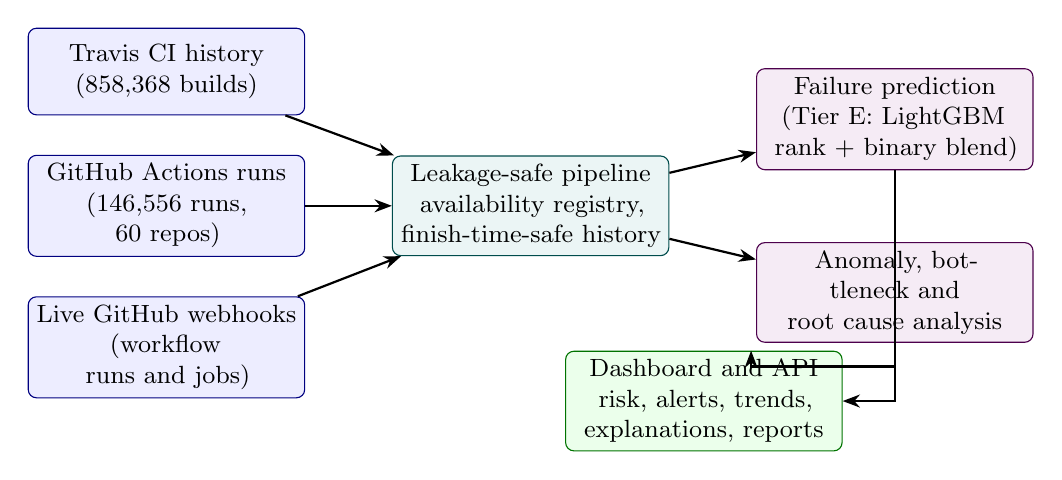
\begin{tikzpicture}[
  font=\small,
  box/.style={draw, rounded corners=3pt, align=center, minimum height=11mm, text width=33mm, inner sep=3pt},
  src/.style={box, fill=blue!7, draw=blue!50!black},
  proc/.style={box, fill=teal!8, draw=teal!60!black},
  ml/.style={box, fill=violet!8, draw=violet!60!black},
  outbox/.style={box, fill=green!8, draw=green!45!black},
  arr/.style={-{Stealth[length=2.2mm]}, thick}]
\node[src] (travis) {Travis~CI history\\(858{,}368 builds)};
\node[src, below=5mm of travis] (gha) {GitHub Actions runs\\(146{,}556 runs, 60 repos)};
\node[src, below=5mm of gha] (live) {Live GitHub webhooks\\(workflow runs and jobs)};
\node[proc, right=11mm of gha] (pipe) {Leakage-safe pipeline\\availability registry,\\finish-time-safe history};
\node[ml, right=11mm of pipe, yshift=11mm] (pred) {Failure prediction\\(\tierE: LightGBM\\rank + binary blend)};
\node[ml, right=11mm of pipe, yshift=-11mm] (diag) {Anomaly, bottleneck and\\root cause analysis};
\node[outbox, below=12mm of pipe, xshift=22mm] (dash) {Dashboard and API\\risk, alerts, trends,\\explanations, reports};
\draw[arr] (travis) -- (pipe);
\draw[arr] (gha) -- (pipe);
\draw[arr] (live) -- (pipe);
\draw[arr] (pipe) -- (pred);
\draw[arr] (pipe) -- (diag);
\draw[arr] (pred.south) |- (dash.east);
\draw[arr] (diag.south) -- ++(0,-3mm) -| ([xshift=6mm]dash.north);
\end{tikzpicture}
\caption{Overview of the AI-driven CI/CD optimization system}
\label{fig:overview}
\end{figure}

The project ``AI-Driven Analysis and Optimization of CI/CD Pipelines for Build Failure Prediction'' addresses these constraints with an intelligent system that predicts build failures and supports pipeline optimization (Fig~\ref{fig:overview}). It combines machine learning, anomaly detection and log analysis to predict build failures before a build runs, recognize slow or stalled pipeline jobs, group recurring failure patterns, and suggest remedies.

The system learns from historical CI/CD data: build outcomes, commits and the size of each change, timing, and the history of each repository, branch and pull request. It was developed on the TravisTorrent dataset~\cite{beller2017travistorrent} of Travis~CI builds and validated on GitHub Actions data that we collected. Random Forest, Decision Tree and Support Vector Machine models from the original plan were trained and compared. The final model is a LightGBM learning-to-rank ensemble that uses the history of the build's own branch or pull request. Anomaly detection identifies jobs that run abnormally long, and log clustering and rule-based diagnosis group similar failures.

\minorhead{Significance of the Project}
The platform helps teams spend a limited review budget where it matters most: it flags the riskiest builds before they run, explains each prediction, and highlights recurring failure types and slow jobs. This can reduce debugging effort and wasted compute and make pipelines more reliable. A visualization dashboard lets developers and administrators observe predictions, failure trends, bottlenecks and suggestions interactively.

The project is significant for software engineering and DevOps for a second reason. It shows how AI methods can support CI/CD processes, and it also shows how such methods must be evaluated before their numbers can be trusted.

\section{Summary of the Work Carried Out}
\label{sec:summarywork}
The project progressed beyond the design proposed in Phase~1 to a complete, evaluated and deployed system:
\begin{itemize}
\item \textbf{Leakage-safe data pipeline.} A registry records when every input becomes available and blocks any input that would only be known after a build finishes. History features count a previous build only once it has finished.
\item \textbf{Prediction models.} Random Forest, Decision Tree, SVM, XGBoost, LightGBM and a stacking ensemble were compared, and a new model (\tierE) was developed that uses the history of each branch or pull request.
\item \textbf{Rigorous evaluation.} Models were evaluated chronologically and \emph{within each repository}, with confidence intervals, and tested on GitHub Actions under protocols written and fixed before the data was collected.
\item \textbf{Deployed system.} A FastAPI service scores GitHub Actions runs automatically through webhooks, issues alerts under a per-repository review budget, detects job bottlenecks and diagnoses failure logs. A React dashboard presents the results, and a read-only public demonstration is available online.
\end{itemize}

\section{Organization of the Report}
\label{sec:organization}
This report is organized into ten chapters.
Chapter 1 introduces the project and its significance.
Chapter 2 presents the problem statement, motivation, objectives and scope.
Chapter 3 reviews existing systems, related research and research gaps.
Chapter 4 outlines the functional, non-functional, hardware and software requirements.
Chapter 5 describes the system design, architecture, methodology and UML diagrams.
Chapter 6 discusses the tools and techniques used.
Chapter 7 describes the implementation: datasets, data pipeline, features, models, the deployed system and the dashboard.
Chapter 8 presents and discusses the results.
Chapter 9 concludes the report and outlines future work.
Chapter 10 lists the references used in the study.

\chapter{Problem Statement}
\label{ch:problem}

\section{Problem Statement}
\label{sec:problem}
Software development today relies heavily on CI/CD pipelines that automate building, testing and deployment. Despite the efficiency and speed they bring, CI/CD pipelines suffer from frequent failures caused by test failures, dependency issues, configuration mismatches, compilation problems, flaky tests and execution instability, which delay software delivery and reduce developer productivity. CI/CD tools such as Jenkins, GitHub Actions and GitLab CI/CD concentrate on executing and observing pipelines. They do not predict likely failures, identify root causes, find bottlenecks, or recommend improvements. Developers must investigate long execution logs to find problems. Moreover, published failure predictors are usually evaluated in ways that leak future information, so their reported accuracy is not what a team would experience. It is therefore reasonable to develop an artificial intelligence-based solution that analyzes CI/CD execution history and predicts failures before a build runs, under an evaluation that matches real use. The same solution should detect abnormal executions, group failure cases, and generate optimization suggestions.

\section{Motivation}
\label{sec:motivation}
CI/CD pipelines are one of the most important aspects of today's DevOps practice because they automate software delivery. While automation increases developer productivity, pipeline failures pose significant challenges. Frequent failures disrupt development work, consume unnecessary computational resources, and delay the delivery of new software.

Finding the error behind a failed pipeline means manually analyzing execution logs, which becomes harder when pipelines have many steps with dependencies between them. Today's CI/CD services focus on automation and monitoring and offer little intelligent analytics.

A second motivation emerged during the project. Build failure prediction looks far easier than it is when it is evaluated carelessly: on our data, the same kind of model scores 0.91 AUC on a random split but only 0.63 when evaluated the way a team would use it (Chapter~\ref{ch:results}). A useful system must therefore be both effective and honestly measured.

This project explores an artificial intelligence-powered CI/CD optimization platform that predicts failures, discovers inefficient pipeline steps, analyzes failure patterns and generates recommendations, all evaluated under a protocol that reflects real use.

\section{Objectives and Scope}
\label{sec:objectives}
\minorhead{Objectives}
\begin{enumerate}
\item Develop a machine learning-based solution that predicts CI/CD pipeline build failures from historical data before the build runs, and evaluate it with a leakage-safe, chronological, within-repository protocol.
\item Detect bottlenecks and abnormal execution behavior in CI/CD pipeline jobs to support pipeline optimization.
\item Provide automated root cause analysis and optimization suggestions to minimize developer debugging effort and improve reliability, presented through an interactive dashboard.
\end{enumerate}

\minorhead{Scope}
This study uses historical CI/CD build data to predict build failures and analyze performance issues. The data covers 858,368 Travis~CI builds from 947 projects (2011--2016) and 146,556 GitHub Actions runs from 60 projects (2025--2026). Machine learning is used to predict failures, and anomaly detection and log analysis are used to find bottlenecks and group failures. The findings are delivered as predictive analytics, bottleneck detection, root cause analysis and optimization suggestions, through an API that receives live GitHub Actions events and a web dashboard. The system is advisory: it never blocks or changes CI builds.

\minorhead{Impact}
For industry, the system helps teams prioritize review and debugging effort and reduce wasted builds. For academia, it provides an evaluation protocol and pre-registered evidence that make build failure prediction results more trustworthy and comparable.

\chapter{Literature Survey}
\label{ch:lit}

\section{Existing Systems}
\label{sec:existing}
Continuous Integration and Continuous Deployment (CI/CD) systems are widely used in modern software development to automate software building, testing and deployment~\cite{hilton2016usage}. They help development teams deliver software faster, reduce manual effort and maintain continuous integration workflows. Popular CI/CD platforms such as Jenkins, GitHub Actions, GitLab CI/CD and Travis CI are used across the software industry.

\textbf{Jenkins} is one of the most widely used open-source CI/CD automation tools. It supports automated builds, testing and deployment through customizable pipelines and plugins. Jenkins automates software delivery efficiently but focuses on execution and monitoring; it cannot predict failures or identify root causes automatically.

\textbf{GitHub Actions} is a cloud-based CI/CD platform integrated directly with GitHub repositories. It automates workflows using YAML configuration files. It improves automation, but developers still inspect logs manually when failures occur, because the platform has no predictive analytics or optimization features.

\textbf{GitLab CI/CD} provides integrated DevOps functionality, including automated testing, deployment, monitoring and repository management, within one platform. It supports scalable delivery workflows but focuses on automation and execution management rather than intelligent prediction and optimization.

\textbf{Travis CI} is commonly used in open-source projects for automated builds and tests. It supports many programming languages and integrates easily with GitHub. However, it offers limited analytics, and failed builds must be debugged manually. Its build histories, published as the TravisTorrent dataset~\cite{beller2017travistorrent}, are the most widely used resource for CI research and are the main development data of this project.

Monitoring and visualization tools such as \textbf{Grafana, Kibana and the ELK Stack} are also widely used to analyze CI/CD logs and execution metrics. They help developers track pipeline performance and visualize trends, but they rely on manual interpretation to identify issues and inefficiencies.

\section{Research on Build Failure Prediction}
\label{sec:research}
Many studies have explored Artificial Intelligence and Machine Learning techniques for CI/CD pipeline management and build failure prediction.

\minorhead{Empirical studies of CI and its failures}
Hilton et al.~\cite{hilton2016usage} studied the usage, costs and benefits of CI in open-source projects and found that CI helps projects release more often but has real costs. Rausch et al.~\cite{rausch2017empirical} conducted a large-scale empirical study of build failures in open-source Java projects and found that test failures cause the majority of broken builds. The study provided useful statistical insights but did not include predictive or optimization mechanisms. Durieux et al.~\cite{durieux2019analysis} analyzed more than 35 million Travis~CI jobs, and later~\cite{durieux2020empirical} studied restarted and flaky builds, identifying unstable tests and network problems as common causes. Gallaba et al.~\cite{gallaba2018noise} showed that historical build data contains noise and heterogeneity, such as failures that are ignored or builds that are restarted, that can mislead analyses. Ghaleb et al.~\cite{ghaleb2019empirical} studied why some CI builds take a long time, which motivates bottleneck detection.

\minorhead{Build outcome prediction}
Hassan and Wang~\cite{hassan2017change} proposed a change-aware build prediction model that uses features of the code change to predict build outcomes and avoid stalls. Ni and Li~\cite{ni2017cost} used cascaded classifiers to predict build outcomes cost-effectively, and Xia and Li~\cite{xia2017could} compared machine learning classifiers for predicting CI build results. Saidani et al.~\cite{saidani2020predicting} used Multi-Objective Genetic Programming on historical build information and software metrics. The study achieved good prediction accuracy but provided no automated root cause analysis or optimization support. Saidani et al.~\cite{saidani2022improving} later applied deep learning models such as LSTM and CNN and improved accuracy over traditional models. However, these models need high computational resources and explain their predictions poorly. Chen et al.\ proposed BuildFast~\cite{chen2020buildfast}, a history-aware predictor that uses the outcomes of previous builds, and Jin and Servant~\cite{jin2020cost} studied cost-efficient approaches that decide which builds to run. Barrak et al.~\cite{barrak2021why} replicated a study of why builds fail using Random Forest models, identifying code complexity, build history and developer activity as important indicators. The system performed poorly on imbalanced data and focused on Java projects. Kumar et al.~\cite{kumar2025optimizing} evaluated models such as Support Vector Machines for predicting build failures from historical pipeline data. Their results were promising, but the work lacked automated root cause analysis and bottleneck detection.

\minorhead{Diagnosis, triage and practice}
Zhang et al.\ proposed BuildSheriff~\cite{zhang2022buildsheriff}, a change-aware triage system that uses stack-trace similarity and code-change analysis to group related test failures and reduce debugging effort. However, the approach mainly supports Java projects in Travis~CI environments and struggles with flaky tests. Hong et al.~\cite{hong2024practitioners} studied practitioners' challenges with, and perceptions of, build failure prediction at Atlassian. They highlight that developers need predictions that are trustworthy and actionable in their own projects. Farihane~\cite{farihane2025ci} presented a systematic mapping study of AI-driven CI/CD pipeline optimization, highlighting the growing use of machine learning for pipeline analytics, failure prediction and automation. That work reviewed existing techniques but did not propose an implementation.

\minorhead{Methodology}
Kaufman et al.~\cite{kaufman2012leakage} formalized \emph{data leakage}: the use of information during training that will not be available when predicting. Bergmeir and Benítez~\cite{bergmeir2012use} discussed how evaluation must respect time order when data are time-dependent. Nosek et al.~\cite{nosek2018preregistration} argued for pre-registration, which means fixing the analysis plan before seeing the data, to make confirmatory results credible. These works shape the evaluation protocol of this project.

\begin{longtable}{|>{\centering\arraybackslash}p{0.7cm}|p{2.9cm}|p{5.6cm}|p{5.0cm}|}
\caption{Literature survey summary}\label{tab:lit}\\
\hline
\textbf{Ref.} & \textbf{Authors (Year)} & \textbf{Method / contribution} & \textbf{Limitation / gap}\\ \hline
\endfirsthead
\hline
\textbf{Ref.} & \textbf{Authors (Year)} & \textbf{Method / contribution} & \textbf{Limitation / gap}\\ \hline
\endhead
\cite{hilton2016usage} & Hilton et al.\ (2016) & Usage, costs and benefits of CI in open source & Descriptive; no prediction\\ \hline
\cite{beller2017travistorrent} & Beller et al.\ (2017) & TravisTorrent dataset of Travis~CI build histories & Mixes pre-build and post-build fields; leakage risk if used naively\\ \hline
\cite{rausch2017empirical} & Rausch et al.\ (2017) & Empirical analysis of build failure causes (Java) & No prediction or optimization\\ \hline
\cite{hassan2017change} & Hassan and Wang (2017) & Change-aware build outcome prediction & No root cause analysis or deployment\\ \hline
\cite{ni2017cost} & Ni and Li (2017) & Cascaded classifiers for cost-effective prediction & Focus on cost; no diagnosis\\ \hline
\cite{xia2017could} & Xia and Li (2017) & Comparison of ML classifiers for CI build results & No diagnosis or deployment\\ \hline
\cite{gallaba2018noise} & Gallaba et al.\ (2018) & Noise and heterogeneity in build data & Descriptive; no prediction\\ \hline
\cite{ghaleb2019empirical} & Ghaleb et al.\ (2019) & Causes of long CI build durations & No prediction\\ \hline
\cite{durieux2019analysis} & Durieux et al.\ (2019) & Analysis of 35M+ Travis~CI jobs & Descriptive; no prediction\\ \hline
\cite{saidani2020predicting} & Saidani et al.\ (2020) & Multi-objective genetic programming for failure prediction & No root cause analysis or optimization\\ \hline
\cite{durieux2020empirical} & Durieux et al.\ (2020) & Restarted and flaky builds on Travis~CI & Focus on flaky builds; no prediction\\ \hline
\cite{chen2020buildfast} & Chen et al.\ (2020) & BuildFast: history-aware outcome prediction & Does not use in-flight build context or pre-registered external tests\\ \hline
\cite{jin2020cost} & Jin and Servant (2020) & Cost-efficient selection of builds to run & Focus on build skipping\\ \hline
\cite{barrak2021why} & Barrak et al.\ (2021) & Random Forest replication of why builds fail & Weak on imbalanced data; Java only\\ \hline
\cite{zhang2022buildsheriff} & Zhang et al.\ (2022) & BuildSheriff: test failure triage by stack-trace similarity & Java/Travis only; struggles with flaky tests\\ \hline
\cite{saidani2022improving} & Saidani et al.\ (2022) & LSTM/CNN deep learning for failure prediction & High compute; limited explainability\\ \hline
\cite{hong2024practitioners} & Hong et al.\ (2024) & Practitioners' perceptions of failure prediction at Atlassian & Qualitative; no new model\\ \hline
\cite{farihane2025ci} & Farihane (2025) & Mapping study of AI for CI/CD optimization & Review only; no implementation\\ \hline
\cite{kumar2025optimizing} & Kumar et al.\ (2025) & SVM and other ML models for failure prediction & No root cause analysis or bottleneck detection\\ \hline
\end{longtable}

\section{Research Gap}
\label{sec:gap}
CI/CD tools prioritize automating and monitoring executions rather than intelligent analytics and optimization. Several papers apply machine learning to detect pipeline failures or analyze logs, but most cover only one part of the problem: some only predict failures, while others only cluster logs or detect anomalies. Very few tools handle prediction, anomaly detection, root cause analysis and optimization together. Existing models also suffer from imbalanced datasets, scalability problems and limited explainability, and most apply only to one CI/CD tool, such as Travis~CI or Jenkins.

During the project, a further and more fundamental gap became clear: \textbf{how results are evaluated}.
\begin{itemize}
\item \textbf{Leakage.} Datasets such as TravisTorrent contain fields computed from the build log (test counts, durations) that encode the outcome. Models that use them look accurate but cannot work before a build runs.
\item \textbf{Random splits.} Shuffling builds lets a model learn a repository's \emph{future} failure rate and use it to predict the past.
\item \textbf{History that ignores finish times.} A build's ``previous outcome'' is only known once that build has finished; using it earlier leaks information.
\item \textbf{Pooled metrics.} Repositories differ greatly in failure rate, so a model can score highly overall just by recognizing risky repositories. That says little about ranking a single team's builds, which is what a team actually needs.
\item \textbf{No confirmatory tests.} Results are rarely re-tested on new data under a plan fixed in advance.
\end{itemize}
There is therefore a need for an AI-based CI/CD optimization solution that combines prediction, anomaly detection, root cause analysis and visualization, and that is evaluated under a protocol matching real use. This project addresses both needs.

\chapter{System Requirement Specification}
\label{ch:srs}

\section{Functional Requirements}
\label{sec:functional}
The artificial intelligence-based pipeline optimization system should satisfy the following functional requirements. Section~\ref{sec:testing} maps each one to its implementation.
\begin{itemize}
\item Collection of historical CI/CD pipeline records, including build outcomes, commits, timing and logs, and live ingestion of GitHub Actions events.
\item Preprocessing and cleansing of pipeline data for effective analysis.
\item Feature extraction from historical records, including code churn, failure rates, commit timing and pipeline history, using only information available before a build runs.
\item Training and execution of machine learning algorithms for build failure prediction.
\item Anomaly detection for slow or abnormal pipeline jobs.
\item Categorization of similar failure logs for automated root cause analysis.
\item Optimization suggestions to improve the efficiency of pipelines.
\item Visualization of pipeline analytics, predictions and bottlenecks through a dashboard.
\end{itemize}

\section{Non-functional Requirements}
\label{sec:nonfunctional}
\begin{itemize}
\item \textbf{Scalability:} The system should cope efficiently with large volumes of CI/CD data from many projects and repositories. Development used 3.56 million Travis~CI job records.
\item \textbf{Reliability:} The platform should produce consistent predictions. The live history computed by the service must equal the history used in training.
\item \textbf{Performance:} The system should score a build quickly enough to be useful before it runs.
\item \textbf{Accuracy:} Models should rank risky builds well within each repository and be evaluated without information leakage.
\item \textbf{Explainability:} Each prediction should come with an explanation of the factors behind it.
\item \textbf{Security:} Webhook endpoints must verify GitHub's HMAC signature, and the public demonstration must be read-only.
\item \textbf{Usability:} The monitoring dashboard should be user-friendly and intuitive.
\item \textbf{Maintainability:} The architecture should make maintenance and enhancement easy; automated tests and continuous integration protect it.
\end{itemize}

\section{Hardware Requirements}
\label{sec:hardware}
\begin{table}[H]
\centering
\caption{Hardware requirements}
\label{tab:hw}
\begin{tabular}{|p{4cm}|p{9cm}|}
\hline
\textbf{Component} & \textbf{Specification}\\ \hline
Processor & Intel i5 / Ryzen 5 / Apple silicon or higher\\ \hline
RAM & Minimum 8 GB (16 GB recommended for training on the full Travis~CI dataset)\\ \hline
Storage & 256 GB SSD\\ \hline
GPU (Optional) & Not required: all models are tree ensembles trained on CPU\\ \hline
Operating System & Windows / Linux / macOS\\ \hline
Deployment & Cloud container service with 512 MB RAM (Render free tier is sufficient for the demonstration)\\ \hline
\end{tabular}
\end{table}

\section{Software Requirements}
\label{sec:software}
\begin{longtable}{|p{4.6cm}|p{8.4cm}|}
\caption{Software requirements}\label{tab:sw}\\
\hline
\textbf{Software Component} & \textbf{Purpose}\\ \hline
\endfirsthead
\hline
\textbf{Software Component} & \textbf{Purpose}\\ \hline
\endhead
Python 3.11 & Core programming language\\ \hline
Pandas, NumPy, PyArrow & Data preprocessing, analysis and storage\\ \hline
Scikit-learn & Random Forest, Decision Tree, SVM, Isolation Forest, TF-IDF and k-means\\ \hline
LightGBM, XGBoost & Gradient-boosted models, including the learning-to-rank model\\ \hline
SHAP & Explanations of individual predictions\\ \hline
FastAPI, Uvicorn & REST API and webhook service\\ \hline
SQLAlchemy, SQLite & Storage of pipelines, builds, predictions and job telemetry\\ \hline
ReportLab & Per-build PDF reports\\ \hline
React, Vite, Tailwind CSS & Web dashboard\\ \hline
Recharts & Animated charts on the dashboard\\ \hline
pytest & Automated tests (84 tests)\\ \hline
GitHub, GitHub Actions & Version control, continuous integration of this project, and a data source\\ \hline
Docker, Render & Containerized deployment of the public demonstration\\ \hline
Visual Studio Code & Development environment\\ \hline
\end{longtable}

\chapter{System Design}
\label{ch:design}

\section{System Architecture}
\label{sec:architecture}
\begin{figure}[H]
\centering
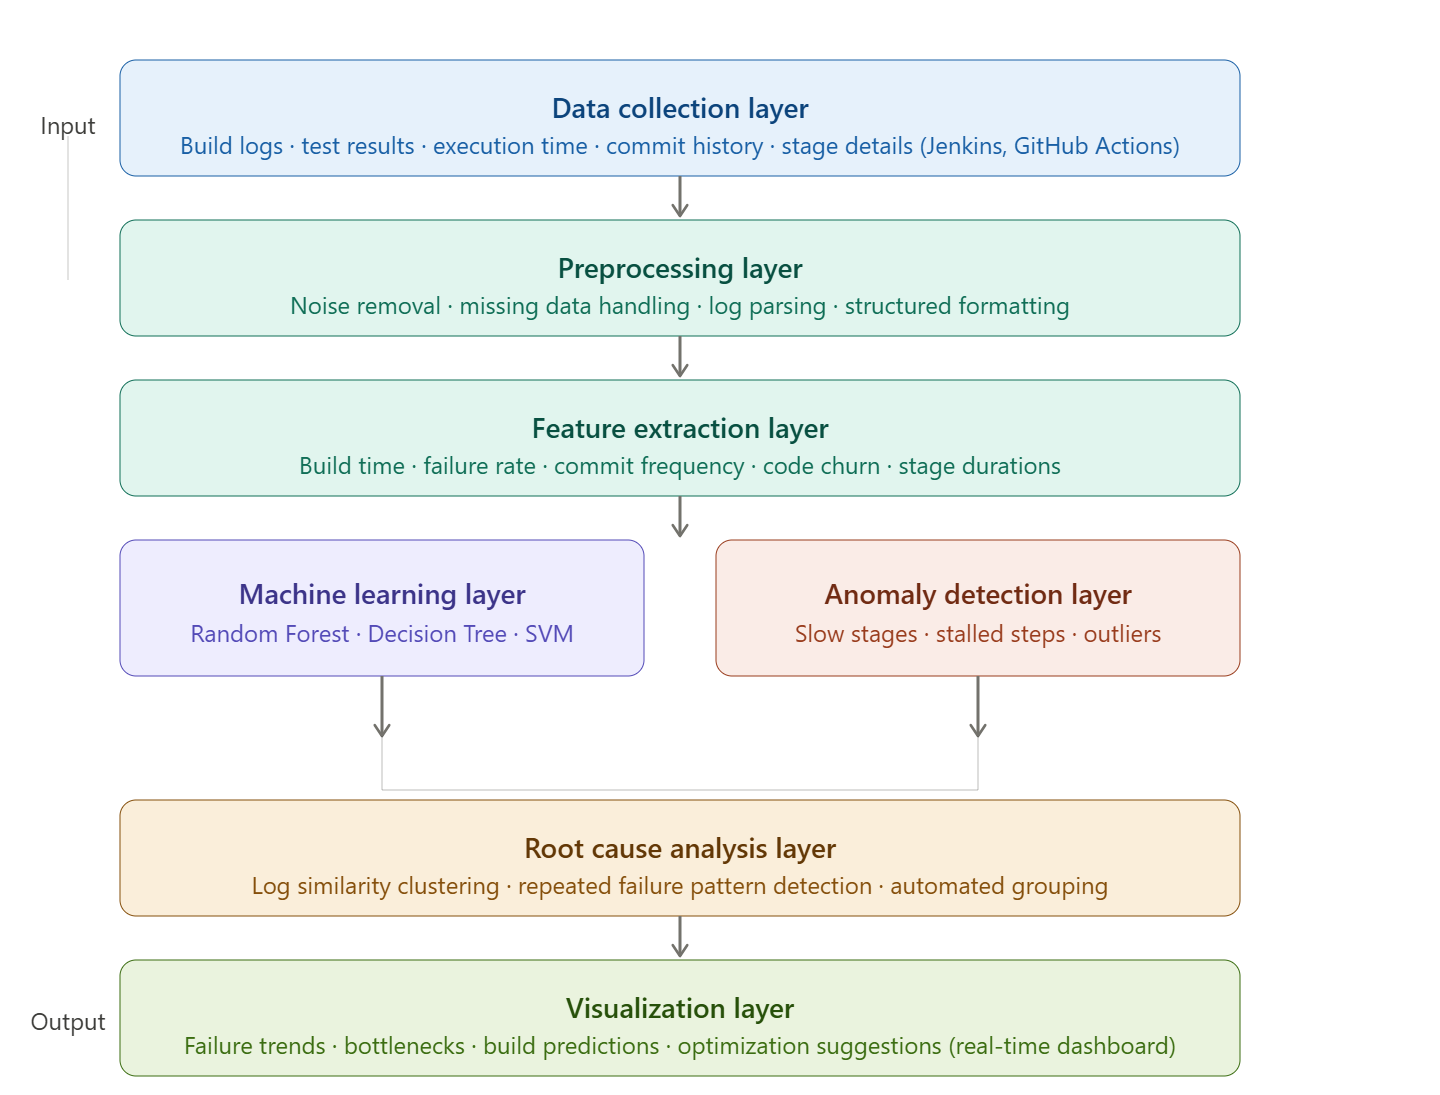
\includegraphics[width=0.92\textwidth]{fig_architecture.png}
\caption{System architecture of the proposed CI/CD optimization framework}
\label{fig:arch}
\end{figure}

The framework uses a modular architecture that analyzes and optimizes CI/CD pipelines through several processing layers (Fig~\ref{fig:arch}). Chapter~\ref{ch:impl} describes how each layer was implemented.
\begin{itemize}
\item \textbf{Data Collection Layer:} Collects historical CI/CD data, including build outcomes, logs, test results, execution times, commit history and job details. The sources are the TravisTorrent export of Travis~CI and the GitHub Actions API. Live data arrives through signed GitHub Actions webhooks, and a Jenkins notification endpoint is also provided.
\item \textbf{Preprocessing Layer:} Cleans and structures the data. It collapses Travis~CI jobs into builds, removes duplicates and re-run attempts, sanitizes logs, and, crucially, enforces when each piece of information becomes available.
\item \textbf{Feature Extraction Layer:} Extracts the size of each change, timing, and the failure history of the repository and of the build's own branch or pull request (its \emph{stream}), using only builds that had finished before the current build started.
\item \textbf{Machine Learning Layer:} Random Forest, Decision Tree and Support Vector Machine were trained as planned, alongside XGBoost, LightGBM and a stacking ensemble. The final model, \tierE, blends a LightGBM classifier with a LightGBM learning-to-rank model.
\item \textbf{Anomaly Detection Layer:} Detects jobs that run abnormally long compared with their own history, and unusual input profiles (Isolation Forest).
\item \textbf{Root Cause Analysis Layer:} Groups similar failure logs (TF-IDF and k-means) and diagnoses failed-job logs with ordered rules, mapping each failure type to a suggestion.
\item \textbf{Visualization Layer:} Displays predictions, alerts, failure trends, bottlenecks, explanations and suggestions on a React dashboard.
\end{itemize}

\section{Proposed Methodology}
\label{sec:methodology}
\begin{figure}[H]
\centering
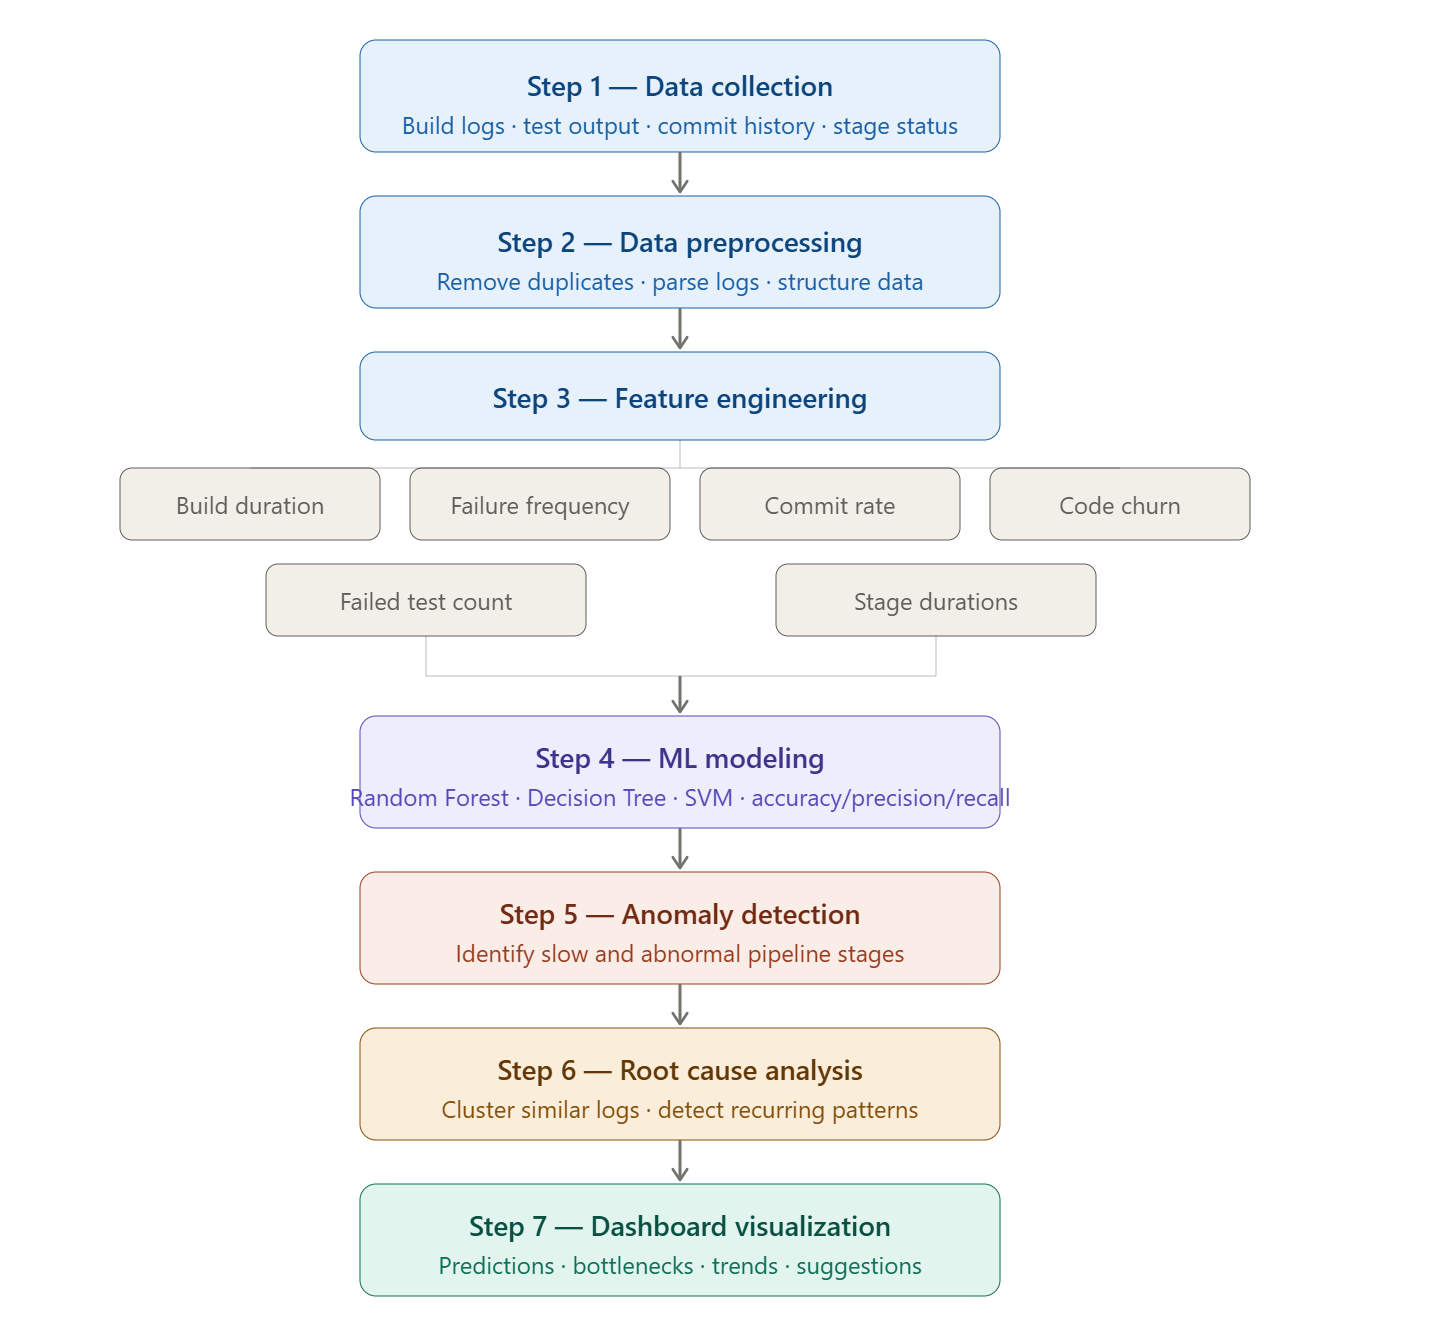
\includegraphics[width=0.78\textwidth]{fig_methodology.png}
\caption{Proposed methodology for AI-driven CI/CD pipeline optimization}
\label{fig:method}
\end{figure}

The solution follows a step-by-step methodology (Fig~\ref{fig:method}): data collection, preprocessing, feature extraction, training of predictive models, bottleneck detection, root cause analysis, and visual dashboard recommendations.

\minorhead{Step 1: Data Collection}
Historical CI/CD data is obtained from TravisTorrent (858,368 Travis~CI builds) and from the GitHub Actions API: workflow runs, their commits, and job timings for 60 public repositories. Live GitHub Actions events arrive through webhooks.

\minorhead{Step 2: Data Preprocessing}
The data is converted to a structured form: jobs are collapsed into builds, duplicates and re-run attempts are removed, unknown completion times are handled, and logs are sanitized. Every input is checked against an \emph{availability registry} that records whether it is known before the build starts.

\minorhead{Step 3: Feature Engineering}
Features that describe the change and its context are extracted from the cleaned data:
\begin{itemize}[label=$\rightarrow$]
\item size of the code change (lines and files changed, by type)
\item failure frequency of the repository, and of the build's own branch or pull request
\item outcome of the previous build, and whether it is still running
\item commit timing and time of day or week
\item number of builds running in the pipeline and started in the last hour
\item job durations, used for bottleneck detection after a build runs
\end{itemize}
Build duration and failed test counts are known only after a build finishes. They are deliberately \emph{not} used to predict failures, because doing so leaks the outcome (Section~\ref{sec:leakage}).

\minorhead{Step 4: Machine Learning Modeling}
Random Forest, Decision Tree, SVM and gradient-boosted models classify whether a build will fail. They are assessed with accuracy, precision, recall and F1, as planned. The primary metric is within-repository AUC under chronological walk-forward evaluation, because it matches how a team would use the predictions.

\minorhead{Step 5: Anomaly Detection}
Slow or stalled jobs are detected by comparing each job's duration with the history of the same job, and unusual input profiles are flagged with Isolation Forest.

\minorhead{Step 6: Root Cause Analysis}
Failure logs are grouped by textual similarity and diagnosed with ordered rules to detect recurring failure patterns. This reduces debugging effort.

\minorhead{Step 7: Dashboard Visualization}
Predictions, alerts, failure trends, bottlenecks and recommendations are presented on an interactive dashboard to help developers analyze pipeline behavior.

\section{Detailed Design}
\label{sec:detailed}

\subsection{Class Diagram}
\label{sec:class}
The detailed design describes the inner workings of, and interactions between, the system's components. Fig~\ref{fig:class} shows the main classes as implemented.

\begin{figure}[H]
\centering
\resizebox{\textwidth}{!}{%
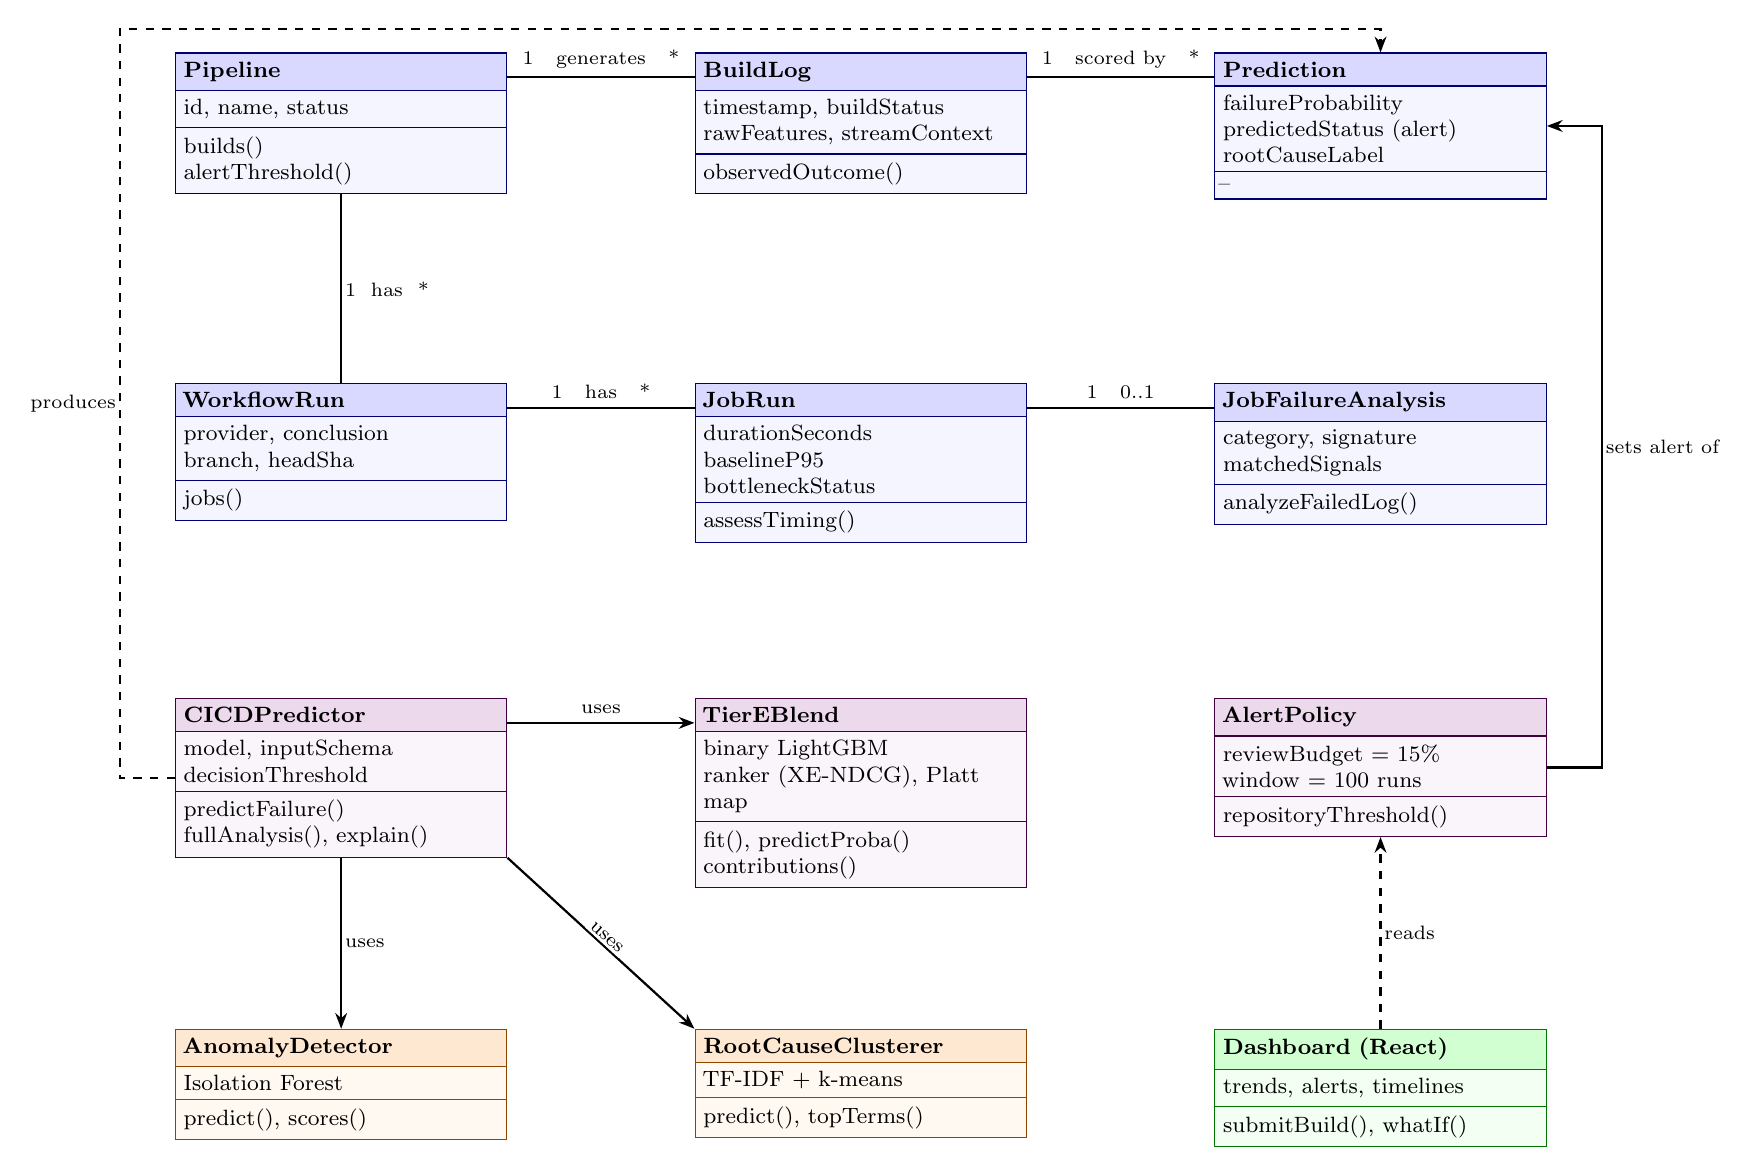
\begin{tikzpicture}[
  font=\footnotesize,
  cls/.style={draw, rectangle split, rectangle split parts=3, align=left, text width=40mm, inner sep=3pt},
  data/.style={cls, draw=blue!45!black, rectangle split part fill={blue!15,blue!4,blue!4}},
  model/.style={cls, draw=violet!50!black, rectangle split part fill={violet!15,violet!4,violet!4}},
  aux/.style={cls, draw=orange!55!black, rectangle split part fill={orange!18,orange!5,orange!5}},
  ui/.style={cls, draw=green!45!black, rectangle split part fill={green!18,green!5,green!5}},
  rel/.style={-{Stealth[length=2mm]}, thick},
  assoc/.style={thick},
  lab/.style={font=\scriptsize, fill=white, inner sep=1pt}]
\def\xa{0} \def\xb{6.6} \def\xc{13.2}
\node[data, anchor=north] (pipe) at (\xa,0) {\textbf{Pipeline}\nodepart{two}id, name, status\nodepart{three}builds()\\alertThreshold()};
\node[data, anchor=north] (build) at (\xb,0) {\textbf{BuildLog}\nodepart{two}timestamp, buildStatus\\rawFeatures, streamContext\nodepart{three}observedOutcome()};
\node[data, anchor=north] (pred) at (\xc,0) {\textbf{Prediction}\nodepart{two}failureProbability\\predictedStatus (alert)\\rootCauseLabel\nodepart{three}--};
\node[data, anchor=north] (wf) at (\xa,-4.2) {\textbf{WorkflowRun}\nodepart{two}provider, conclusion\\branch, headSha\nodepart{three}jobs()};
\node[data, anchor=north] (job) at (\xb,-4.2) {\textbf{JobRun}\nodepart{two}durationSeconds\\baselineP95\\bottleneckStatus\nodepart{three}assessTiming()};
\node[data, anchor=north] (fa) at (\xc,-4.2) {\textbf{JobFailureAnalysis}\nodepart{two}category, signature\\matchedSignals\nodepart{three}analyzeFailedLog()};
\node[model, anchor=north] (cp) at (\xa,-8.2) {\textbf{CICDPredictor}\nodepart{two}model, inputSchema\\decisionThreshold\nodepart{three}predictFailure()\\fullAnalysis(), explain()};
\node[model, anchor=north] (te) at (\xb,-8.2) {\textbf{TierEBlend}\nodepart{two}binary LightGBM\\ranker (XE-NDCG), Platt map\nodepart{three}fit(), predictProba()\\contributions()};
\node[model, anchor=north] (ap) at (\xc,-8.2) {\textbf{AlertPolicy}\nodepart{two}reviewBudget = 15\%\\window = 100 runs\nodepart{three}repositoryThreshold()};
\node[aux, anchor=north] (ad) at (\xa,-12.4) {\textbf{AnomalyDetector}\nodepart{two}Isolation Forest\nodepart{three}predict(), scores()};
\node[aux, anchor=north] (rc) at (\xb,-12.4) {\textbf{RootCauseClusterer}\nodepart{two}TF-IDF + k-means\nodepart{three}predict(), topTerms()};
\node[ui, anchor=north] (dash) at (\xc,-12.4) {\textbf{Dashboard (React)}\nodepart{two}trends, alerts, timelines\nodepart{three}submitBuild(), whatIf()};
\draw[assoc] (pipe.east |- build.text) -- node[lab, above=2pt]{1 \ \ generates \ \ *} (build.west |- build.text);
\draw[assoc] (build.east |- pred.text) -- node[lab, above=2pt]{1 \ \ scored by \ \ *} (pred.west |- pred.text);
\draw[assoc] (pipe.south) -- node[lab, right]{1 \ has \ *} (wf.north);
\draw[assoc] (wf.east |- job.text) -- node[lab, above=2pt]{1 \ \ has \ \ *} (job.west |- job.text);
\draw[assoc] (job.east |- fa.text) -- node[lab, above=2pt]{1 \ \ 0..1} (fa.west |- fa.text);
\draw[rel] (cp.east |- te.text) -- node[lab, above=2pt]{uses} (te.west |- te.text);
\draw[rel] (cp.south) -- node[lab, right]{uses} (ad.north);
\draw[rel] (cp.south east) -- node[lab, above, sloped]{uses} (rc.north west);
\draw[rel] (ap.east) -- ++(0.7,0) |- node[lab, pos=0.25, right]{sets alert of} (pred.east);
\draw[rel, dashed] (cp.west) -- ++(-0.7,0) |- node[lab, pos=0.25, left]{produces} ([yshift=3mm]pred.north) -- (pred.north);
\draw[rel, dashed] (dash.north) -- node[lab, right]{reads} (ap.south);
\end{tikzpicture}}
\caption{Class diagram of the CI/CD optimization system}
\label{fig:class}
\end{figure}

\begin{itemize}
\item \textbf{Data classes.} \texttt{Pipeline} represents a repository. A \texttt{BuildLog} stores one build or workflow run, its observed outcome and the stream history derived for it, and each \texttt{Prediction} stores its risk, alert decision and root cause. \texttt{WorkflowRun} and \texttt{JobRun} store job telemetry used for bottleneck detection, and \texttt{JobFailureAnalysis} stores the diagnosis of a failed job's log.
\item \textbf{Prediction classes.} \texttt{CICDPredictor} loads the deployed model and scores builds using \texttt{TierEBlend}. \texttt{AlertPolicy} turns a score into an alert using the repository's own review budget.
\item \textbf{Analysis classes.} \texttt{AnomalyDetector} and \texttt{RootCauseClusterer} provide anomaly detection and log clustering.
\item \textbf{Dashboard.} The React dashboard presents the results to the user.
\end{itemize}
The design originally included a \texttt{User} class with login. Sign-in was later removed: the dashboard is an internal or read-only tool, and machine endpoints are protected by webhook signatures and shared secrets instead.

\subsection{Activity Diagram}
\label{sec:activity}
\begin{figure}[H]
\centering
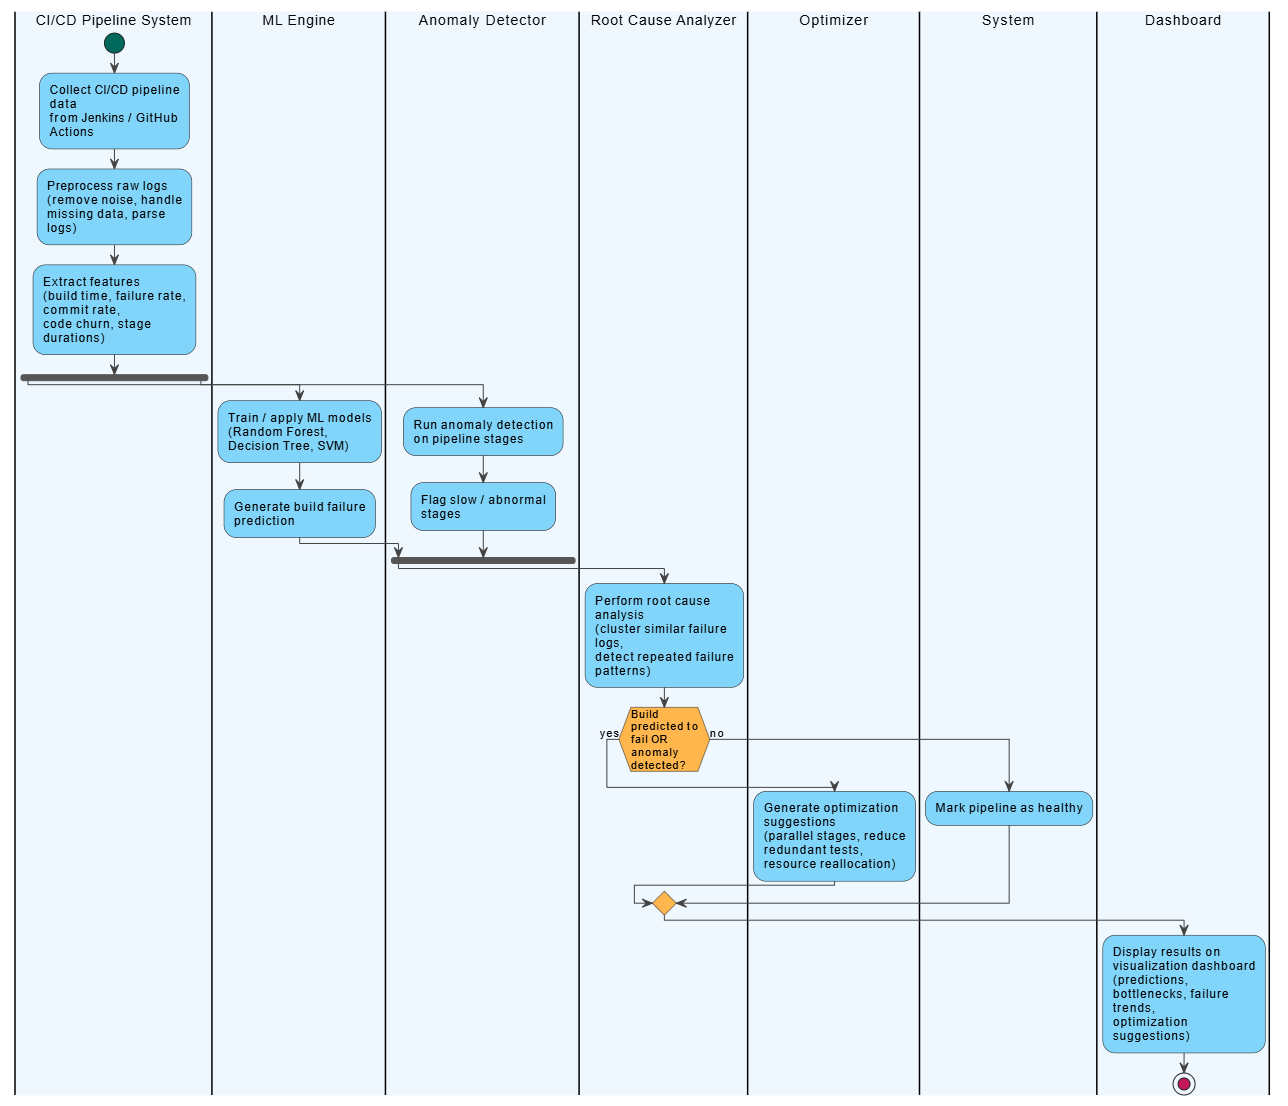
\includegraphics[width=\textwidth]{fig_activity.png}
\caption{Activity diagram of the CI/CD optimization system}
\label{fig:activity}
\end{figure}
The activity diagram depicts the flow of events in the system (Fig~\ref{fig:activity}).
\begin{enumerate}
\item CI/CD pipeline data is gathered from repositories and build systems.
\item The data is preprocessed and passed to feature engineering.
\item Machine learning models produce build failure predictions. In the deployed system this happens when a GitHub Actions run is requested, before it executes.
\item The anomaly detection and root cause analysis components detect bottlenecks and recurring failure patterns.
\item When a build is predicted to fail or an anomaly is found, optimization suggestions are generated.
\item Finally, the results are displayed on the dashboard.
\end{enumerate}

\subsection{Use Case Diagram}
\label{sec:usecase}
\begin{figure}[H]
\centering
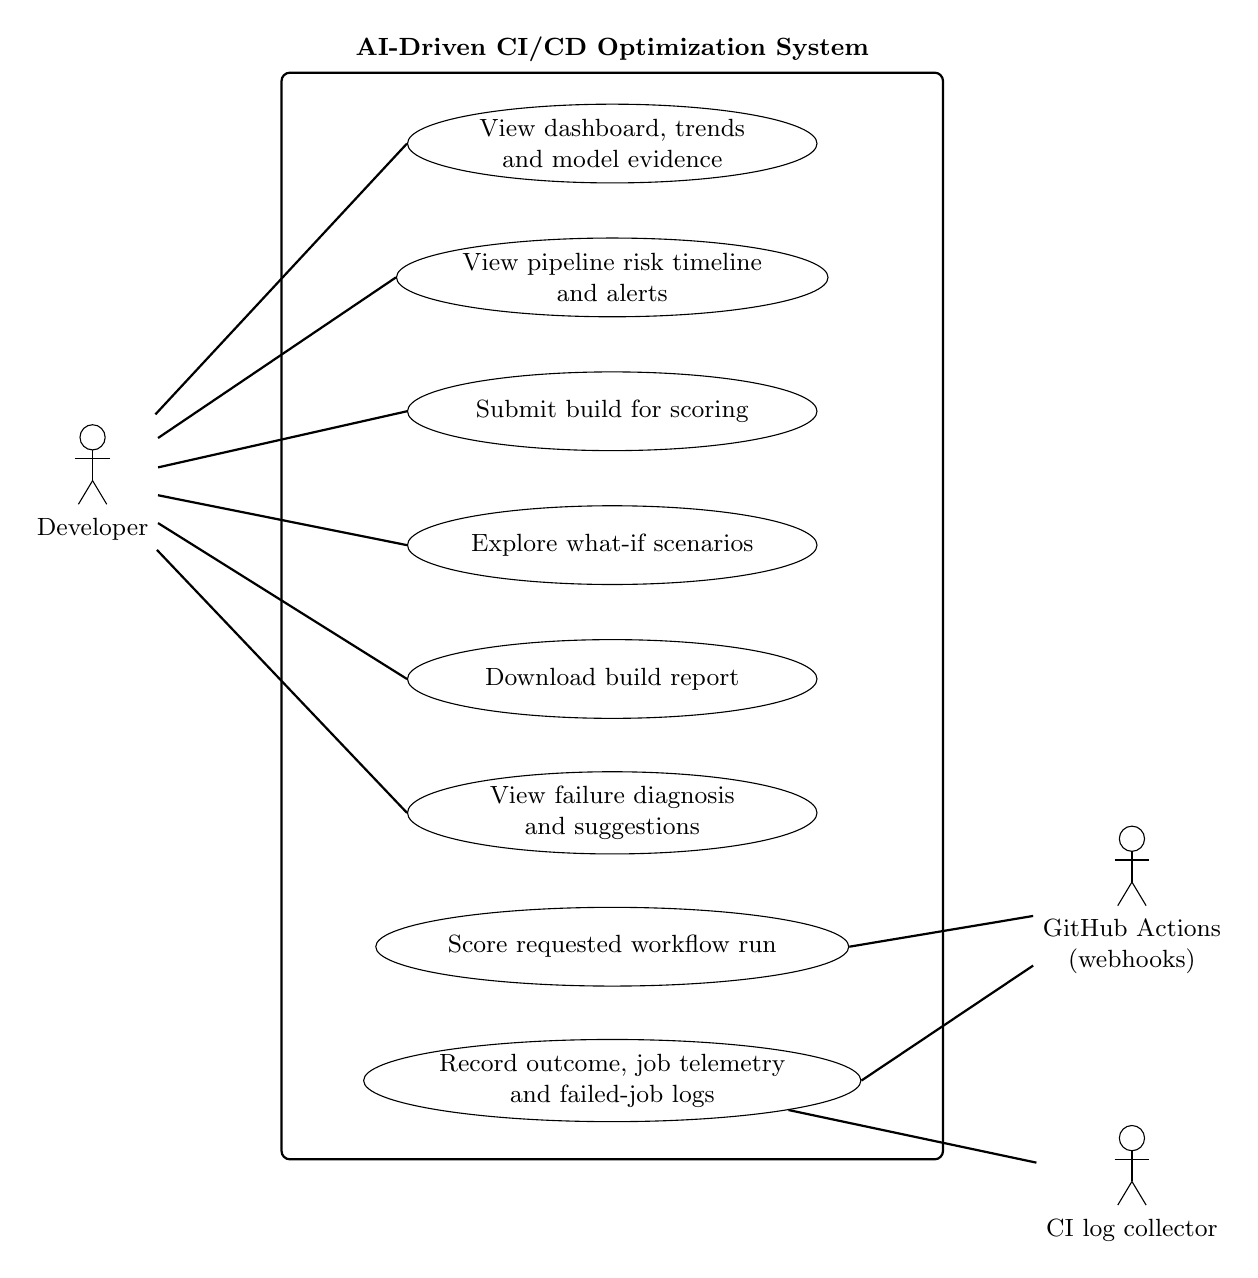
\begin{tikzpicture}[
  font=\small,
  uc/.style={draw, ellipse, align=center, minimum width=52mm, minimum height=10mm, inner sep=1pt, fill=white},
  actor/.style={align=center, font=\small},
  link/.style={thick}]
\node[draw, thick, rounded corners=3pt, minimum width=84mm, minimum height=138mm, label={[font=\small\bfseries]above:AI-Driven CI/CD Optimization System}] (sys) at (0,0) {};
\foreach \name/\y/\txt in {u1/6.0/{View dashboard, trends\\and model evidence}, u2/4.3/{View pipeline risk timeline\\and alerts}, u3/2.6/{Submit build for scoring}, u4/0.9/{Explore what-if scenarios}, u5/-0.8/{Download build report}, u6/-2.5/{View failure diagnosis\\and suggestions}, u7/-4.2/{Score requested workflow run}, u8/-5.9/{Record outcome, job telemetry\\and failed-job logs}}
  \node[uc] (\name) at (0,\y) {\txt};
\newcommand{\stick}{\tikz{\draw (0,0.45) circle (0.16); \draw (0,0.29) -- (0,-0.1); \draw (-0.22,0.18) -- (0.22,0.18); \draw (0,-0.1) -- (-0.18,-0.4); \draw (0,-0.1) -- (0.18,-0.4);}}
\node[actor] (dev) at (-6.6,1.7) {\stick\\Developer};
\node[actor] (gh) at (6.6,-3.6) {\stick\\GitHub Actions\\(webhooks)};
\node[actor] (col) at (6.6,-7.2) {\stick\\CI log collector};
\foreach \u in {u1,u2,u3,u4,u5,u6} \draw[link] (dev) -- (\u.west);
\draw[link] (gh) -- (u7.east);
\draw[link] (gh) -- (u8.east);
\draw[link] (col) -- (u8.south east);
\end{tikzpicture}
\caption{Use case diagram of the CI/CD optimization system}
\label{fig:usecase}
\end{figure}

The use case diagram (Fig~\ref{fig:usecase}) shows how users and external systems interact with the solution.

\minorhead{Actors}
\begin{itemize}
\item \textbf{Developer:} views the dashboard, pipelines and alerts, scores builds and explores what-if scenarios.
\item \textbf{GitHub Actions:} sends signed workflow-run and job events.
\item \textbf{CI log collector:} an optional workflow that uploads failed-job logs.
\end{itemize}

\minorhead{Use Cases}
\begin{itemize}
\item View dashboard, failure trends and model evidence
\item View a pipeline's risk timeline and alerts
\item Submit a build for scoring
\item Explore what-if scenarios
\item Download a per-build PDF report
\item View failure diagnosis and optimization suggestions
\item Score a requested workflow run automatically
\item Record run outcomes, job telemetry and failed-job logs
\end{itemize}

\chapter{Identification of Tools and Techniques}
\label{ch:tools}

\section{Development Tools}
\label{sec:devtools}
The system uses tools chosen for scalability, compatibility, and their support for machine learning, data analysis and pipeline integration.

\textbf{Python 3.11} is the primary programming language, chosen for its simplicity, cross-platform support and extensive ecosystem of machine learning and data processing libraries. All package versions are pinned so that saved model artifacts load exactly as trained.

\textbf{Scikit-learn}~\cite{pedregosa2011scikit} implements Random Forest, Decision Tree and Support Vector Machine for build failure prediction, along with Isolation Forest, TF-IDF and k-means for anomaly detection and log clustering, and the evaluation metrics.

\textbf{LightGBM}~\cite{ke2017lightgbm} and \textbf{XGBoost}~\cite{chen2016xgboost} provide gradient-boosted trees. LightGBM also provides the learning-to-rank objective used by the final model.

\textbf{Pandas, NumPy and PyArrow} are used for data preprocessing, cleaning, feature extraction, numerical computation and efficient storage of the 3.56 million-row Travis~CI data.

\textbf{SHAP}~\cite{lundberg2017unified} explains individual predictions by attributing each prediction to its input features.

\textbf{Visual Studio Code} is the main development environment, and \textbf{pytest} runs the automated test suite.

Deep learning frameworks (TensorFlow, PyTorch) were planned for possible future use. They were not needed: tree ensembles performed well, are faster to train, and are easier to explain.

\section{CI/CD and Integration Tools}
\label{sec:citools}
\textbf{GitHub Actions} is a cloud-based CI/CD platform tightly coupled with GitHub repositories. In this project it plays three roles:
\begin{itemize}
\item \textbf{Data source:} workflow runs, commits and job timings of 60 public repositories were collected through its API.
\item \textbf{Live input:} the deployed system receives signed \texttt{workflow\_run} and \texttt{workflow\_job} webhook events and scores each run when it is requested.
\item \textbf{CI for this project:} every pull request runs the backend tests and a production build of the dashboard.
\end{itemize}

\textbf{Travis~CI}, through the TravisTorrent dataset~\cite{beller2017travistorrent}, provides the main development data: 3.56 million job records from 947 projects.

\textbf{Jenkins} is one of the most widely used open-source CI/CD automation servers. The system provides a Jenkins notification endpoint protected by a shared secret, so Jenkins builds can be recorded and scored as well.

\textbf{GitHub} hosts the project's code and is used for version control, pull requests and releases. Commit activity on GitHub, such as code churn, files changed and commit timing, also provides important model features.

\section{Visualization and Deployment Tools}
\label{sec:viztools}
The design originally proposed Grafana and Kibana for visualization. Instead, a purpose-built \textbf{React} dashboard was implemented with \textbf{Vite}, \textbf{Tailwind CSS} and \textbf{Recharts}. It shows exactly the project's outputs: failure risk, alerts, trends, explanations, bottlenecks and model evidence. It uses animated, colorblind-checked charts, and every chart has a legend or labels. The backend is a \textbf{FastAPI} service with a \textbf{SQLite} database (via SQLAlchemy). \textbf{ReportLab} generates per-build PDF reports.

\textbf{Docker} packages the service. A read-only public demonstration runs as a single container on \textbf{Render}, serving the dashboard and the API from one address.

\section{Techniques Used}
\label{sec:techniques}

\minorhead{Random Forest}
Random Forest~\cite{breiman2001random} is an ensemble of decision trees trained on random subsets of data and features. It is robust against overfitting and handles mixed, complex features well. In this project it is the main baseline: \tierC, a Random Forest with repository history, is the model that \tierE\ is compared against.

\minorhead{Decision Tree}
A Decision Tree~\cite{quinlan1986induction} classifies data with a hierarchy of decision rules derived from the features. It is interpretable, which helps explain what drives pipeline failures. It was trained and compared as planned.

\minorhead{Support Vector Machine (SVM)}
SVM~\cite{cortes1995support} finds the boundary that best separates classes in a high-dimensional feature space. It was evaluated against Random Forest and Decision Tree using accuracy, precision, recall and F1-score.

\minorhead{Gradient Boosting and Learning to Rank}
Gradient boosting (XGBoost~\cite{chen2016xgboost}, LightGBM~\cite{ke2017lightgbm}) builds trees sequentially, each correcting the errors of the previous ones. A team's real question is ``which of \emph{our} builds are riskiest?'', so the final model also uses a \emph{learning-to-rank} objective, XE-NDCG~\cite{bruch2021alternative}. It learns to order builds within each repository and month rather than to classify them in isolation. Platt scaling~\cite{platt1999probabilistic} converts the blended score into a probability.

\minorhead{SHAP Explanations}
SHAP values~\cite{lundberg2017unified} attribute each prediction to its input features, such as ``the previous run of this workflow failed'' or ``many lines changed''. The dashboard shows them as red (raises risk) and blue (lowers risk) bars.

\minorhead{Anomaly and Bottleneck Detection}
Bottleneck detection compares a job's duration with at least 10 earlier runs of the same job. A job is flagged when it exceeds both their 95th percentile and a robust threshold of the median plus three median absolute deviations. Isolation Forest~\cite{liu2008isolation} flags unusual pre-build input profiles. It is not a failure predictor: in testing, anomalous builds did not fail more often, so the dashboard does not present it as one.

\minorhead{Log Clustering and Diagnosis}
Failure logs are represented with TF-IDF term weights~\cite{salton1988term} and grouped with k-means clustering~\cite{lloyd1982least}, so that similar failures fall in the same group (Fig~\ref{fig:logflow}). Failed-job logs from GitHub Actions are also sanitized and matched against ordered diagnostic rules, which report the matched lines and suggest a fix. The categories are resource or runner exhaustion, timeouts and network instability, dependency or build-configuration failures, compilation errors, and test assertion failures.

\begin{figure}[H]
\centering
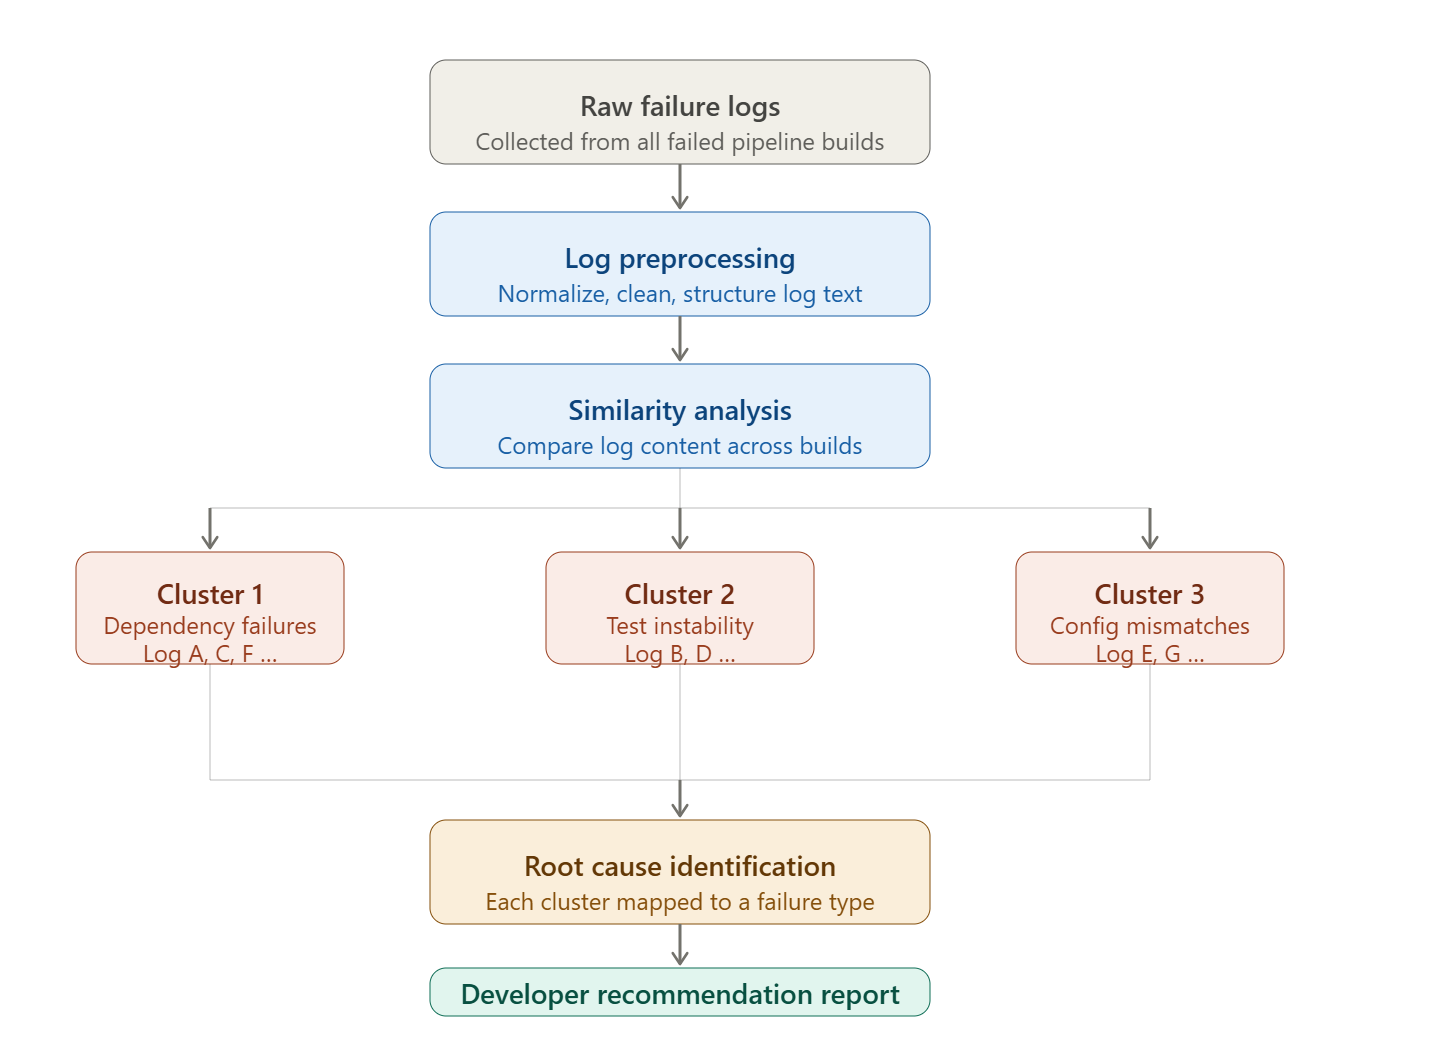
\includegraphics[width=0.78\textwidth]{fig_overview.png}
\caption{Log clustering flow for root cause analysis}
\label{fig:logflow}
\end{figure}

\minorhead{Feature Engineering}
Meaningful attributes are extracted from raw CI/CD data: code churn, files changed by type, failure rates of the repository and of the build's branch or pull request, the outcome of the previous build, builds still running, and commit timing. Every feature is checked against the availability registry, so nothing that is only known after a build finishes can be used (Section~\ref{sec:pipeline}).

\minorhead{Leakage-Safe Evaluation}
Models are evaluated with chronological walk-forward folds: they are trained only on the past and tested on the future. The metric is AUC measured within each repository, and confidence intervals come from bootstrapping over repositories~\cite{efron1993introduction}. External tests were pre-registered~\cite{nosek2018preregistration}: their plan was fixed and fingerprinted before any data was collected.

\chapter{Implementation}
\label{ch:impl}

\section{Datasets}
\label{sec:datasets}
Three datasets were used (Table~\ref{tab:data}).

\minorhead{Travis~CI (development)}
The TravisTorrent export~\cite{beller2017travistorrent} contains 3.56 million job records. A Travis build runs several jobs, for example on different language versions. We collapsed the jobs into \textbf{858,368 builds} from \textbf{947 projects} (April~2011 to August~2016), checking that every pre-build field is identical across a build's jobs. A build fails if any of its jobs failed; 19.5\% of builds failed. A build's finish time is its start time plus its longest job's duration. Missing durations are filled with the repository's 95th-percentile duration.

\minorhead{GitHub Actions (external tests)}
On GitHub Actions the unit is a \emph{workflow run}. We kept first attempts of \texttt{push} and \texttt{pull\_request} runs. \texttt{success} is a pass, and \texttt{failure} and \texttt{startup\_failure} are failures; cancelled and skipped runs are excluded. A run's finish time is its \texttt{updated\_at}, and runs whose completion time is unknown are dropped. The size of each change (lines added and deleted, files changed, message length, parents) comes from the commits API.

The \emph{first} GitHub Actions dataset covers 30 repositories. The \emph{confirmation} dataset was collected with our own collector under a protocol fixed in advance. It takes the first 30 eligible repositories from a search of popular repositories, excluding all repositories used before, with runs created between 15~August and 30~September~2026. Of the qualifying runs, 3,773 (4.6\%) were dropped because their commits, mostly on deleted forks, could no longer be fetched.

\begin{table}[H]
\centering
\caption{Datasets used in the project}
\label{tab:data}
\begin{tabular}{|l|r|r|r|l|}
\hline
\textbf{Dataset} & \textbf{Builds / runs} & \textbf{Repos} & \textbf{Failure rate} & \textbf{Period}\\ \hline
Travis~CI (TravisTorrent) & 858,368 & 947 & 19.5\% & 2011--2016\\ \hline
GitHub Actions, test 1 & 67,980 & 30 & 8.9\% & 2025--2026\\ \hline
GitHub Actions, confirmation & 78,576 & 30 & 28.2\% & Aug--Sep 2026\\ \hline
GitHub Actions, combined & 146,556 & 60 & 19.2\% & 2025--2026\\ \hline
\end{tabular}
\end{table}

\section{Leakage-Safe Data Pipeline}
\label{sec:pipeline}
Most of the effort went into making sure that no model ever sees information it would not have when a build is triggered.

\minorhead{Availability registry}
Every column is recorded in a versioned registry with the stage at which it becomes known: pre-build, build start, or post-build. Fields computed from the build log, such as test counts, test duration and build duration, are marked post-build. So are comment counts, which can be written after the build. The predictor checks its inputs against the registry when it starts and refuses to run if any input is not available at prediction time.

\minorhead{Finish-time-safe history}
History features count a previous build only if it \emph{finished} strictly before the current build was triggered. Builds are processed per repository in time order, with a queue of builds still running; a build's outcome enters the history only once its finish time has passed. Ties are broken by finish time, then trigger time, then build id. In every evaluation run, a brute-force recomputation re-checks the history values on sampled repositories, and a deliberately leaked feature makes this check fail.

\minorhead{Finish buffers}
To test robustness, outcomes can be withheld for an extra 1 or 6 hours after a build finishes, which simulates delays in reporting.

\section{Feature Engineering}
\label{sec:features}
Features are organized in tiers (Table~\ref{tab:tiers}). A \emph{stream} is the build's pull request or, for push builds, its branch. On GitHub Actions, runs carry no pull request number, so a pull request is identified by its author and head branch.

{\renewcommand{\arraystretch}{1.3}
\begin{longtable}{|p{1.6cm}|p{12.2cm}|}
\caption{Feature tiers}\label{tab:tiers}\\
\hline
\textbf{Tier} & \textbf{Features}\\ \hline
\endfirsthead
\hline
\textbf{Tier} & \textbf{Features}\\ \hline
\endhead
Tier~A & \textbf{The change and its context} (18 features): source and test churn; files added, deleted and modified by type; hour, day, month, weekend and night flags; pull request flag; core-team author; default branch; and the project language. On GitHub Actions: lines added and deleted, files changed, message length, merge commit, default branch, and the workflow.\\ \hline
Tier~C & Tier~A plus \textbf{project context} (team size, code size, test density, past commits on the touched files, commits in the build) and \textbf{repository history}: the previous finished build's outcome and the repository's failure rate over the last 5 builds and overall.\\ \hline
Tier~E & Tier~C plus \textbf{stream history}: the outcome of the stream's last finished build; the stream's last-5 and overall failure rates, finished-build count and failure streak; the outcome of the build's predecessor (on Travis, the previous build on the branch; on GitHub Actions, the previous run of the same workflow on the stream); and an exponentially weighted repository failure rate.\newline
It also adds \textbf{in-flight context}: whether the previous build and the stream's last build are still running, how many builds are running in the repository, how many started in the last hour, and the hours since the stream last triggered. In-flight features use only the existence and start times of earlier builds, never their outcomes.\\ \hline
\end{longtable}}

\section{Prediction Models}
\label{sec:models}
\minorhead{Planned classifiers}
As planned, Random Forest, Decision Tree and SVM were trained, alongside XGBoost, LightGBM and a stacking ensemble (Random Forest, XGBoost and LightGBM combined by logistic regression). Hyperparameters were tuned with randomized search (25 settings, 3-fold cross-validation, F1 score) on a 200,000-row sample. The comparison is reported in Section~\ref{sec:leakage} as a \emph{development reference only}, because it uses a random split.

\minorhead{Final model: \tierE}
The final model combines two LightGBM models trained on \tierE\ features:
\begin{itemize}
\item a binary classifier, which predicts whether a build fails;
\item a ranker trained with the XE-NDCG objective~\cite{bruch2021alternative}, which learns to order builds within one repository and calendar month (one ranking ``query'').
\end{itemize}
Let $b(x)$ be the classifier's log-odds and $r(x)$ the ranker's score. Both are standardized with the mean and standard deviation of the \emph{training} scores and averaged:
\begin{equation}
s(x) = \tfrac{1}{2}\,\frac{r(x)-\mu_r}{\sigma_r} + \tfrac{1}{2}\,\frac{b(x)-\mu_b}{\sigma_b}.
\end{equation}
A Platt map~\cite{platt1999probabilistic} fitted on training scores turns $s(x)$ into a probability. LightGBM settings were fixed before any confirmation data was scored: 600 trees, learning rate 0.03, 63 leaves, at least 200 samples per leaf, 80\% row and column sampling, and L2 regularization 1.0.

\minorhead{Deployed model}
The deployed model is trained on walk-forward folds 1--9 of the 146,556 GitHub Actions runs, with the newest 10\% held out. Before it is saved, it must reproduce the research evaluation's predictions on the held-out fold; the largest difference was 0. Explanations use SHAP values of the binary half of the model.

\section{Anomaly, Bottleneck and Root Cause Modules}
\label{sec:aux}
\begin{itemize}
\item \textbf{Bottleneck detection.} For every completed GitHub Actions job, the system compares its duration with at least 10 earlier runs of the same job. A job that exceeds both their 95th percentile and the median plus three median absolute deviations is marked as a bottleneck. A scheduled collector also checks jobs that are still running, so stalled jobs are flagged while they run.
\item \textbf{Anomaly detection.} An Isolation Forest (10\% contamination) flags builds whose pre-build input profile is unusual. Because such builds did not fail more often, the flag is kept as a diagnostic and not shown as a failure prediction.
\item \textbf{Root cause analysis.} Failed-test text is clustered with TF-IDF and k-means. Failed GitHub Actions job logs, uploaded by an optional workflow, are sanitized and diagnosed with ordered rules into five categories. Each category maps to a suggestion, for example retrying transient tests and mocking external calls, or pinning compatible dependency versions.
\end{itemize}

\section{Deployed System}
\label{sec:deployed}
\begin{figure}[H]
\centering
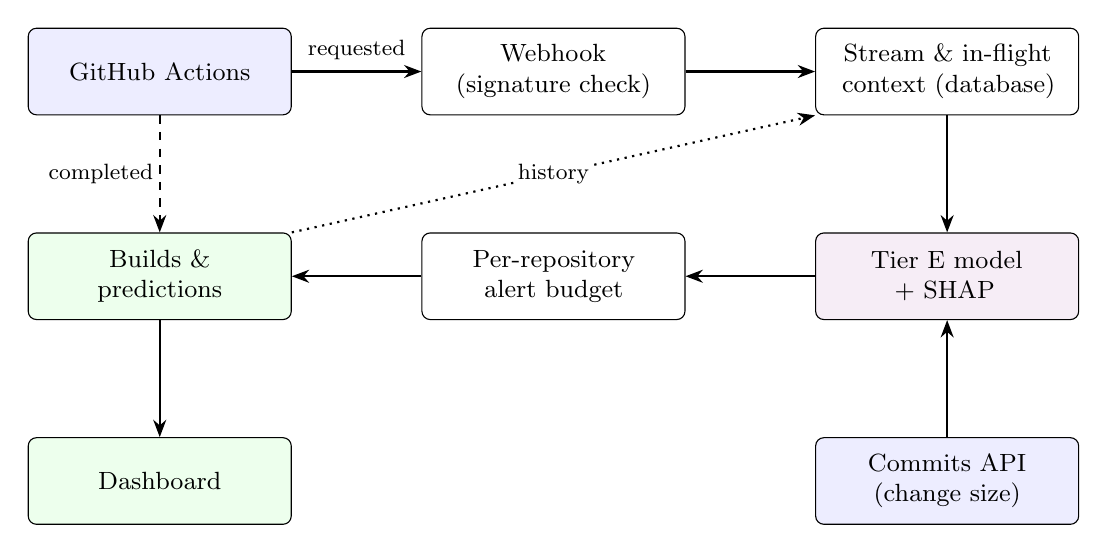
\begin{tikzpicture}[
  font=\small,
  box/.style={draw, rounded corners=3pt, align=center, minimum height=11mm, text width=32mm, inner sep=2pt, fill=white},
  arr/.style={-{Stealth[length=2.2mm]}, thick},
  lab/.style={font=\footnotesize, fill=white, inner sep=1pt}]
\node[box, fill=blue!7] (gh) at (0,0) {GitHub Actions};
\node[box] (hook) at (5,0) {Webhook\\(signature check)};
\node[box] (ctx) at (10,0) {Stream \& in-flight\\context (database)};
\node[box, fill=green!7] (db) at (0,-2.6) {Builds \&\\predictions};
\node[box] (alert) at (5,-2.6) {Per-repository\\alert budget};
\node[box, fill=violet!7] (model) at (10,-2.6) {\tierE\ model\\+ SHAP};
\node[box, fill=green!7] (ui) at (0,-5.2) {Dashboard};
\node[box, fill=blue!7] (cmt) at (10,-5.2) {Commits API\\(change size)};
\draw[arr] (gh) -- node[lab, above=3pt] {requested} (hook);
\draw[arr] (hook) -- (ctx);
\draw[arr] (ctx) -- (model);
\draw[arr] (model) -- (alert);
\draw[arr] (alert) -- (db);
\draw[arr] (db) -- (ui);
\draw[arr] (cmt) -- (model);
\draw[arr, dashed] (gh) -- node[lab, left=1pt] {completed} (db);
\draw[arr, dotted] (db.north east) -- node[lab] {history} (ctx.south west);
\end{tikzpicture}
\caption{Scoring path of the deployed system}
\label{fig:scoring}
\end{figure}

\minorhead{Scoring path}
Fig~\ref{fig:scoring} shows the scoring path. A FastAPI service receives signed GitHub \texttt{workflow\_run} events.
\begin{enumerate}
\item When a run is \emph{requested}, before it executes, the service builds the run's stream history and in-flight context from the repository's stored runs, and fetches the commit's size from the GitHub API.
\item It scores the run with \tierE\ and stores a shadow prediction with its explanation.
\item When the run \emph{completes}, its real outcome is attached and becomes history for later runs. Other conclusions, such as cancelled runs, are stored but never become history, as in training.
\end{enumerate}
Runs are timed by GitHub's own creation and completion times, so a late webhook delivery cannot change a run's history. The system is advisory and never blocks CI.

\minorhead{Same history live as in training}
Automated tests replay synthetic run histories through both the offline training pass and the live service, and check that every history and in-flight value matches, row by row.

\minorhead{Per-repository alert budget}
A single global threshold flags too many runs in risky repositories and almost none in safe ones. Instead, a run becomes an alert when its risk reaches the 85th percentile of its \emph{own repository's} last 100 scored runs: each repository reviews its riskiest 15\%. Until a repository has 20 scored runs, a ``typical repository'' threshold of 0.893 is used. Neither threshold uses outcome labels. Section~\ref{sec:alerts} evaluates this policy.

\minorhead{Public demonstration}
A read-only demonstration runs on Render as a single Docker container that serves the dashboard and the API from one address. It replays 450 real GitHub Actions runs from \texttt{twbs/bootstrap}, \texttt{freeCodeCamp} and \texttt{yt-dlp} through the real webhook, at their real times. The runs come from the model's held-out period, so every prediction shown is out-of-sample, and contributor and branch names are replaced with pseudonyms. Visitors can explore every page and score builds, but nothing is saved.

\section{Dashboard}
\label{sec:dashboard}
The dashboard has four pages.

\minorhead{Dashboard}
Summary cards, the daily trend of average predicted risk against the actual failure rate (Fig~\ref{fig:dash_overview}), the distribution of predicted risk, and a model-evidence panel with the research results (Fig~\ref{fig:dash_models}, Chapter~\ref{ch:results}).

\begin{figure}[H]
\centering
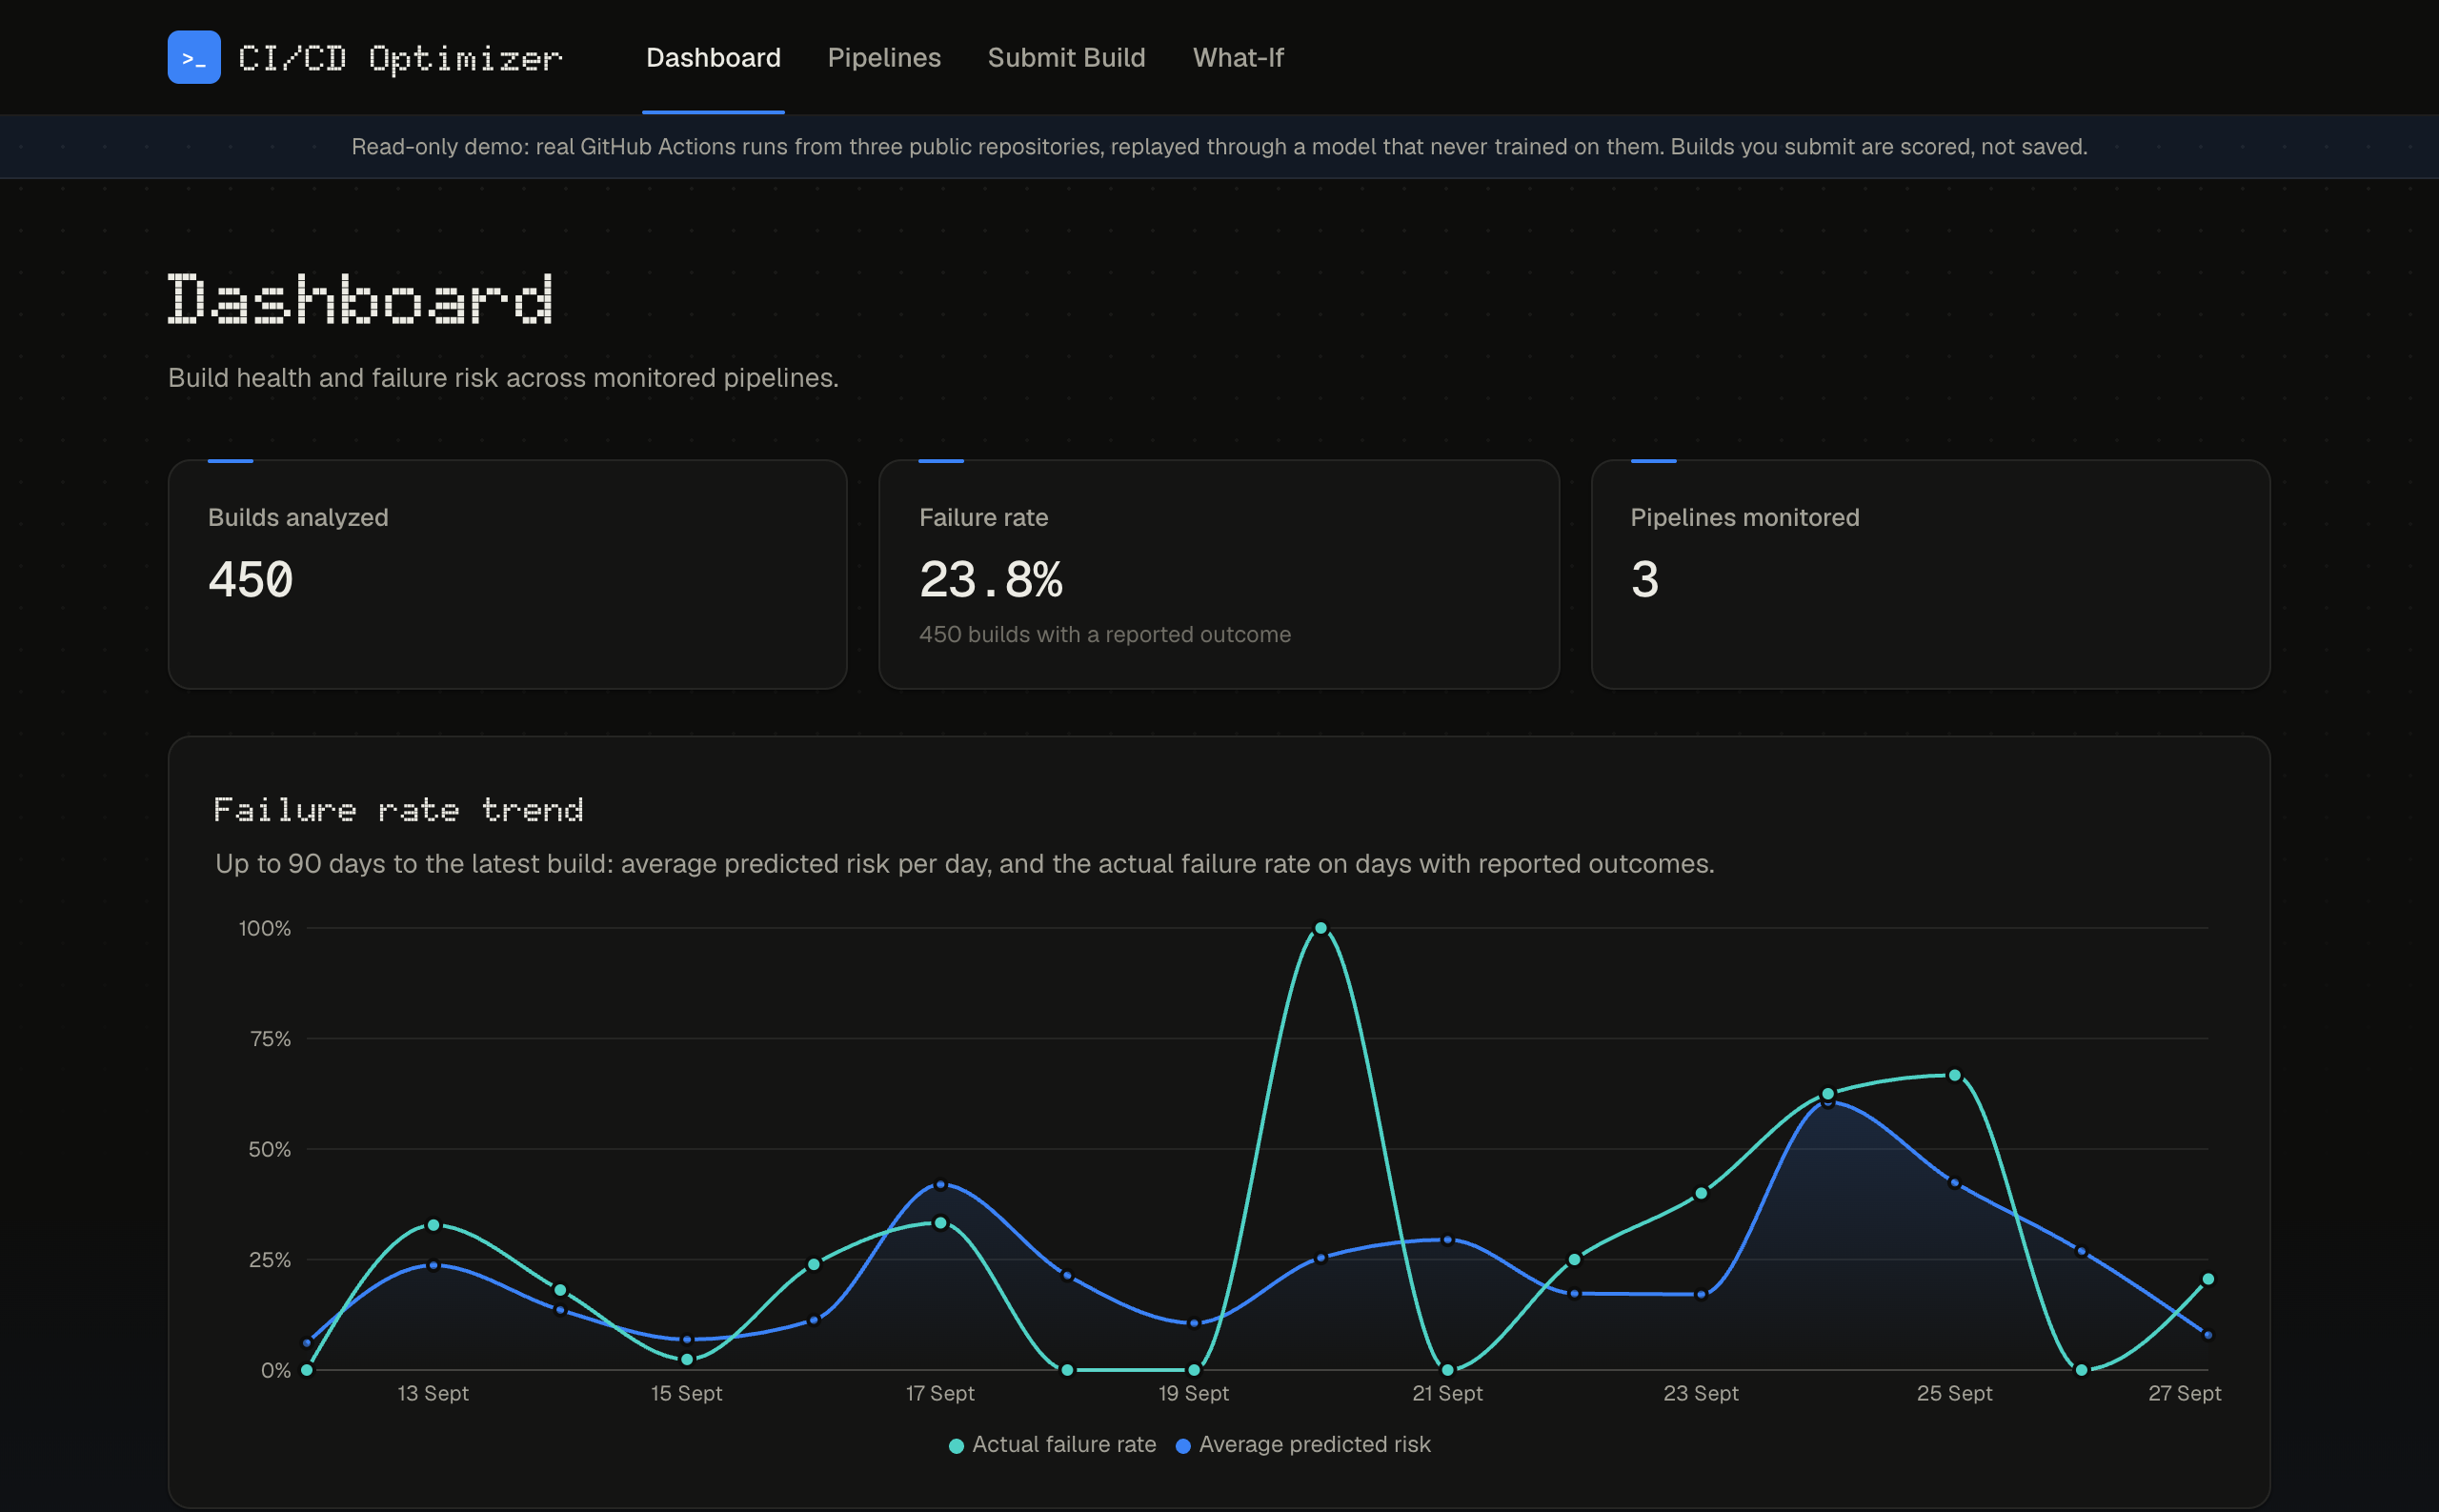
\includegraphics[width=0.92\textwidth]{dashboard_overview.png}
\caption{Dashboard: summary cards and daily failure-rate trend (public demonstration)}
\label{fig:dash_overview}
\end{figure}

\minorhead{Pipelines}
Each repository's latest status and risk, with a sparkline of its recent risk (Fig~\ref{fig:pipelines}). A repository's page shows its risk over time, with each run colored by its real outcome and the repository's alert threshold as a dashed line (Fig~\ref{fig:timeline}). It also lists every build with its explanation and a downloadable PDF report.

\begin{figure}[H]
\centering
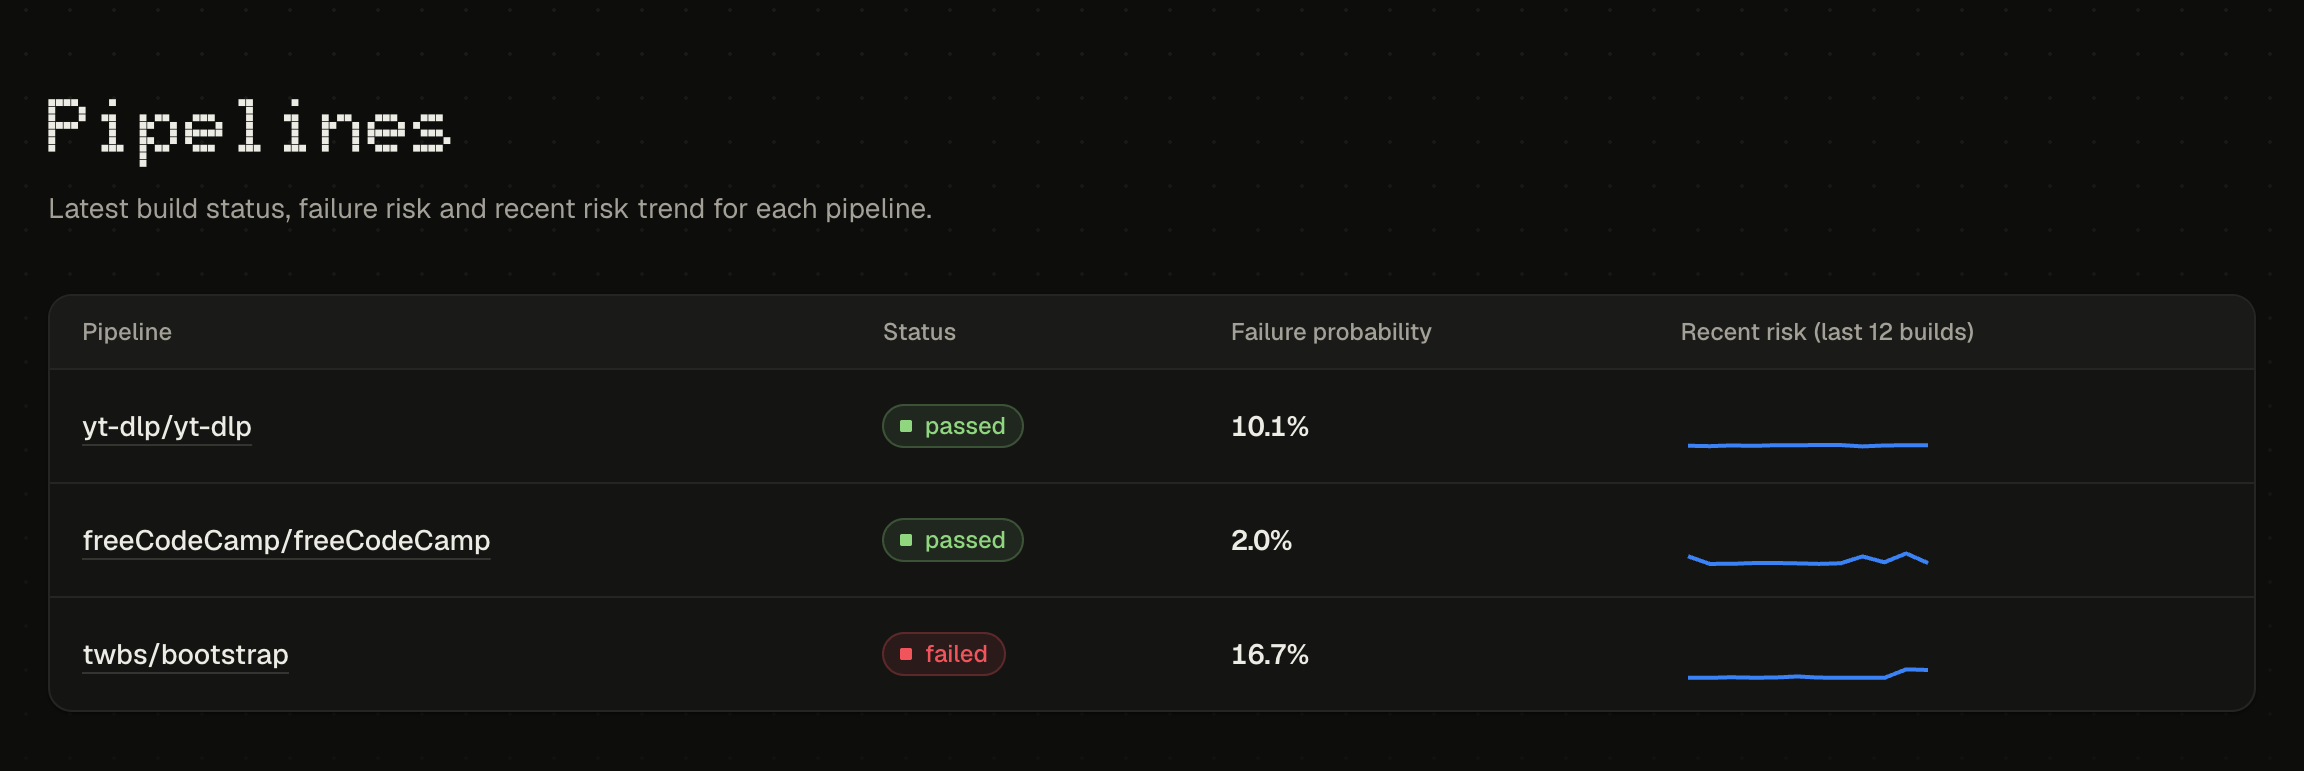
\includegraphics[width=0.92\textwidth]{pipelines.png}
\caption{Pipelines page with recent-risk sparklines}
\label{fig:pipelines}
\end{figure}

\begin{figure}[H]
\centering
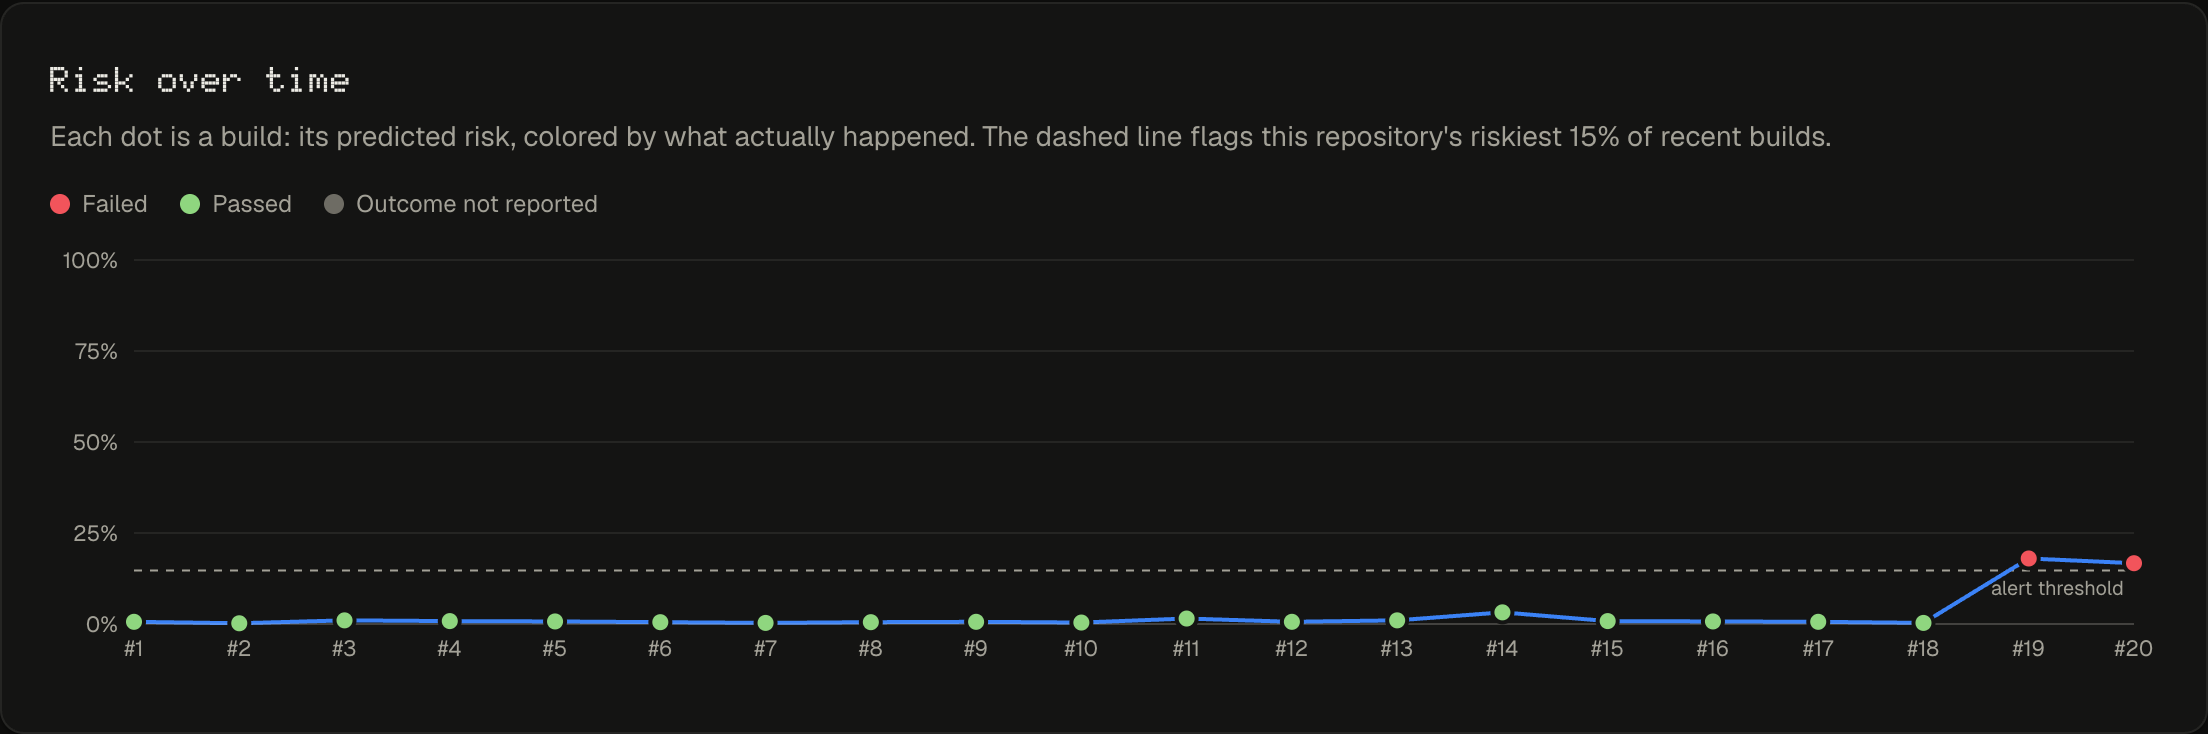
\includegraphics[width=\textwidth]{pipeline_timeline.png}
\caption{Risk timeline of \texttt{twbs/bootstrap}. The two newest runs, both real failures, rise above the repository's alert threshold.}
\label{fig:timeline}
\end{figure}

\minorhead{Submit Build}
Scores a GitHub Actions run described by its repository, workflow, pull request author and branch, and commit size. It shows the history the server derived for it and compares the risk with the repository's own threshold (Fig~\ref{fig:submit}).

\begin{figure}[H]
\centering
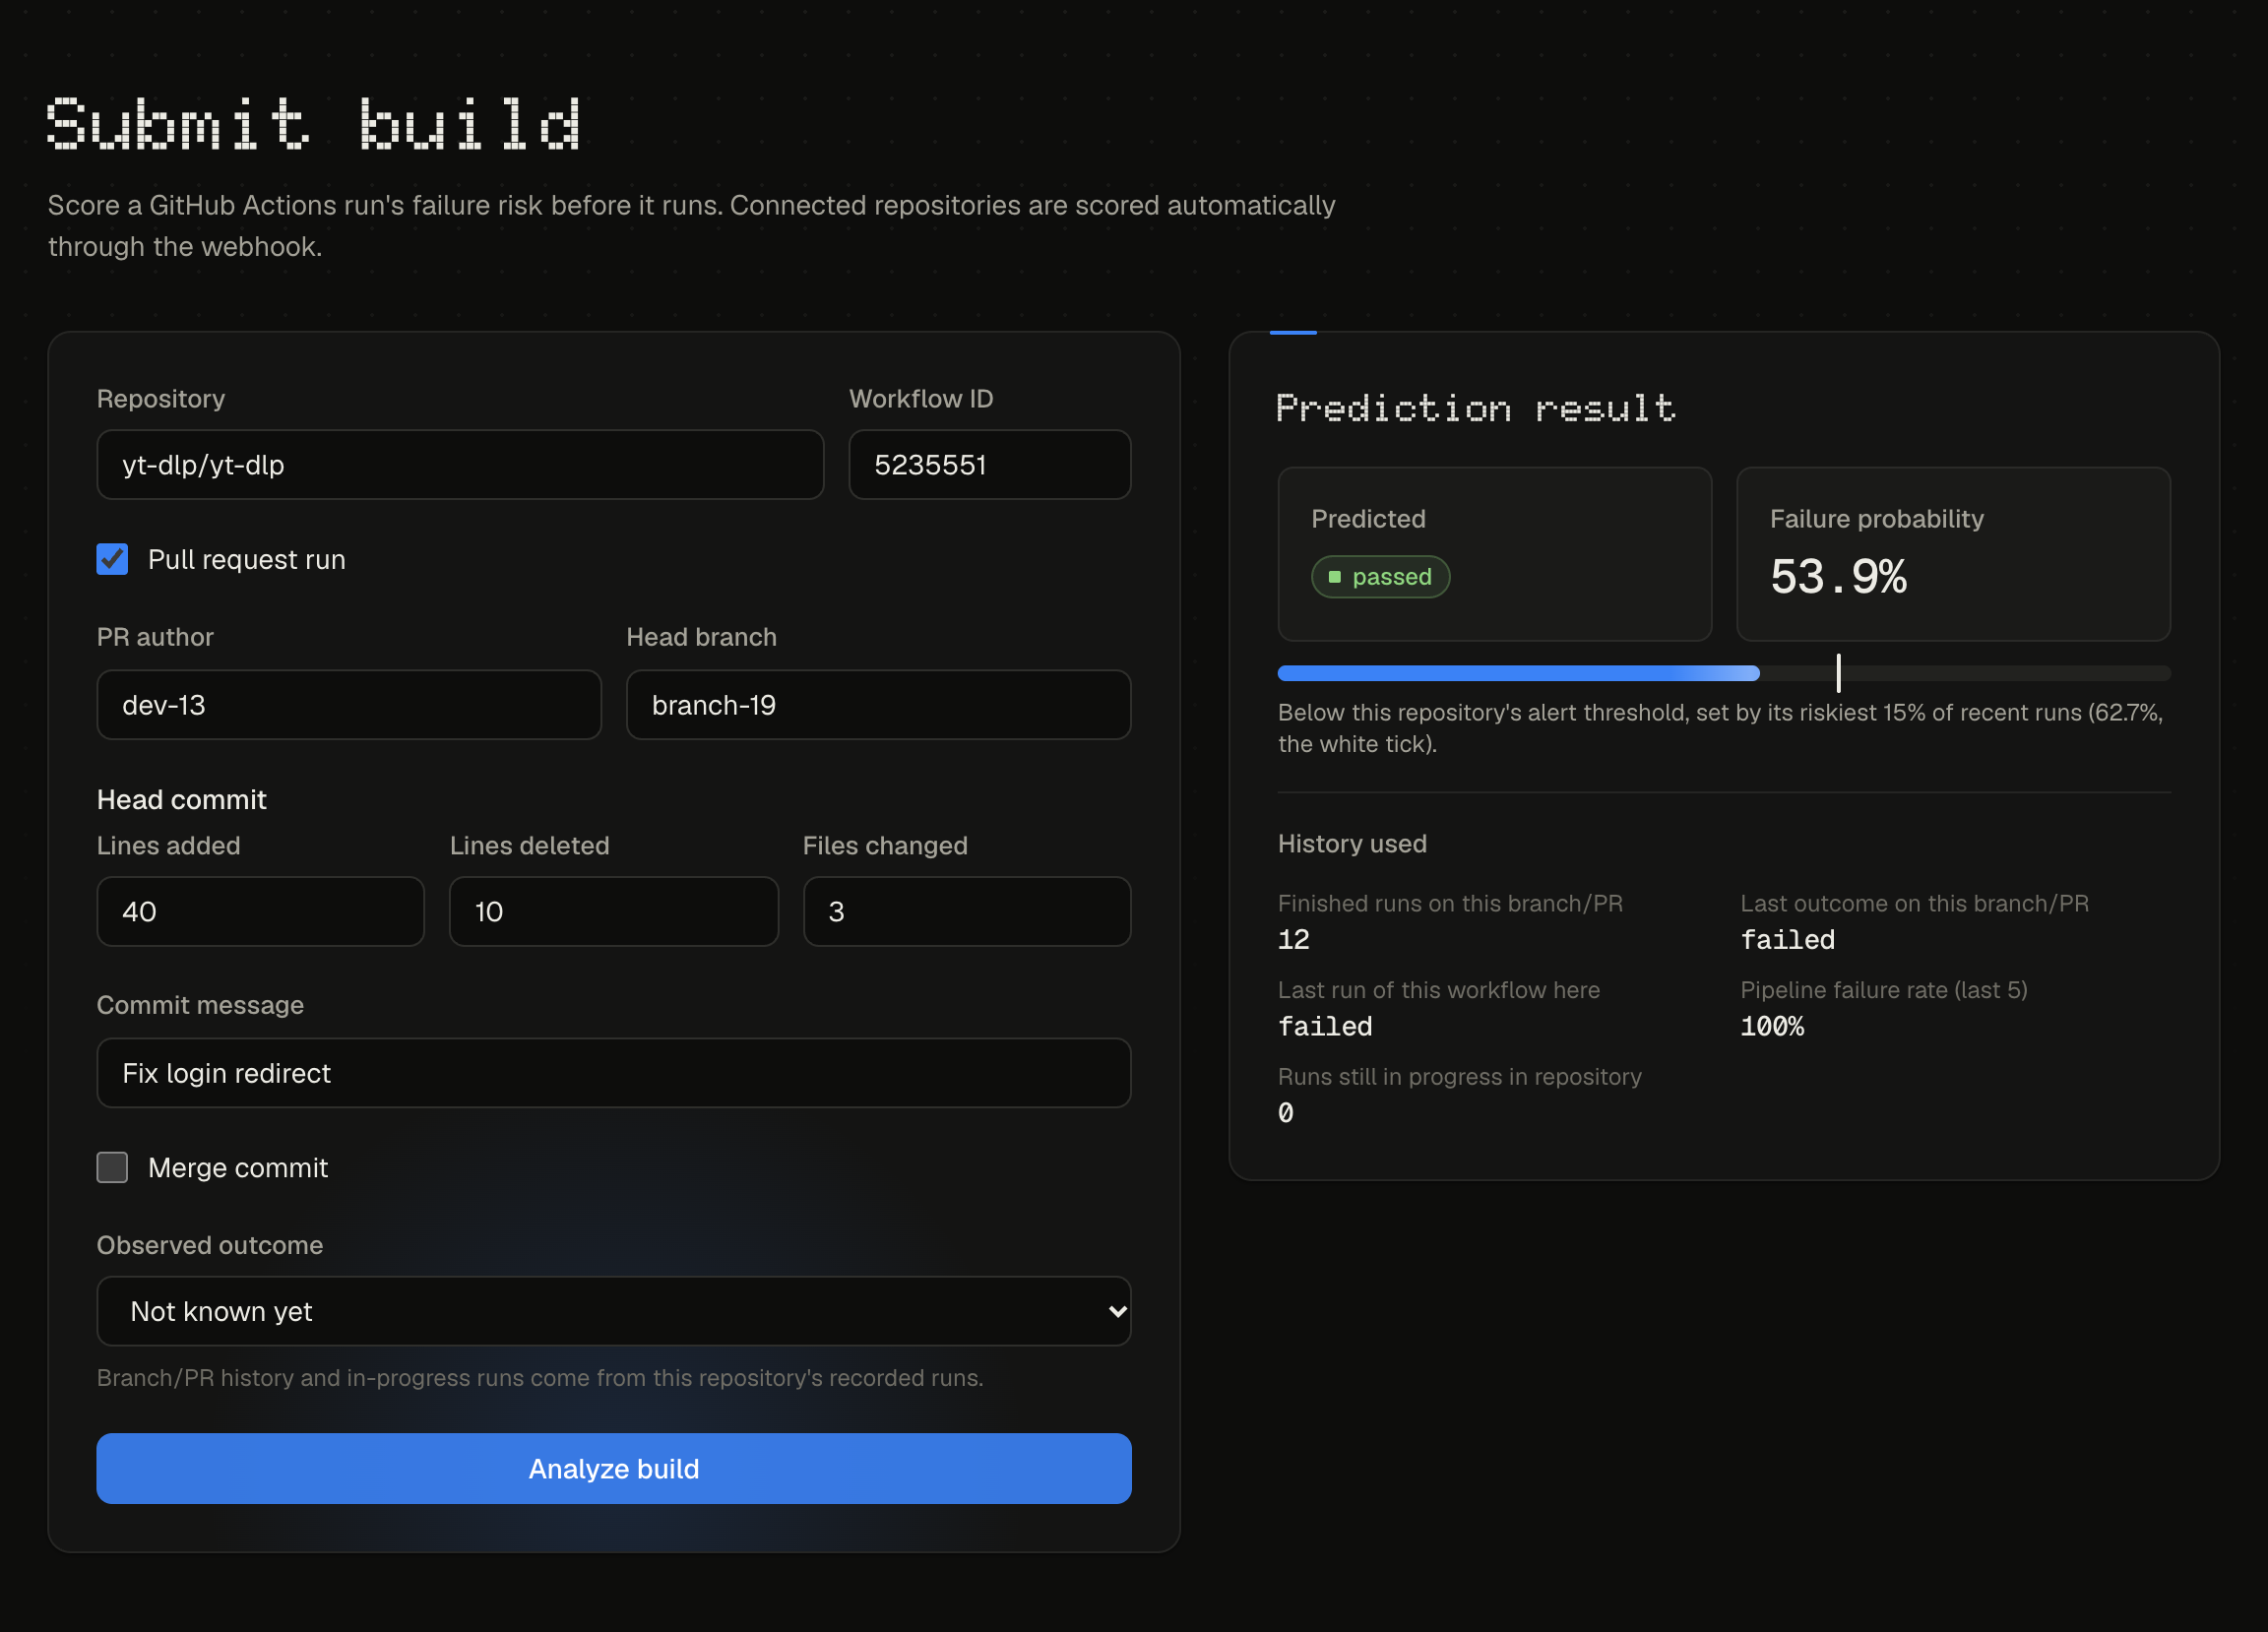
\includegraphics[width=0.9\textwidth]{submit_result.png}
\caption{Submit Build: a run on a failing \texttt{yt-dlp} branch, scored with server-derived history}
\label{fig:submit}
\end{figure}

\minorhead{What-If}
Changes inputs and immediately shows how the risk moves, with SHAP explanations and a trail of the risk across edits (Fig~\ref{fig:whatif}). An optimization simulation compares one changed input against the baseline.

\begin{figure}[H]
\centering
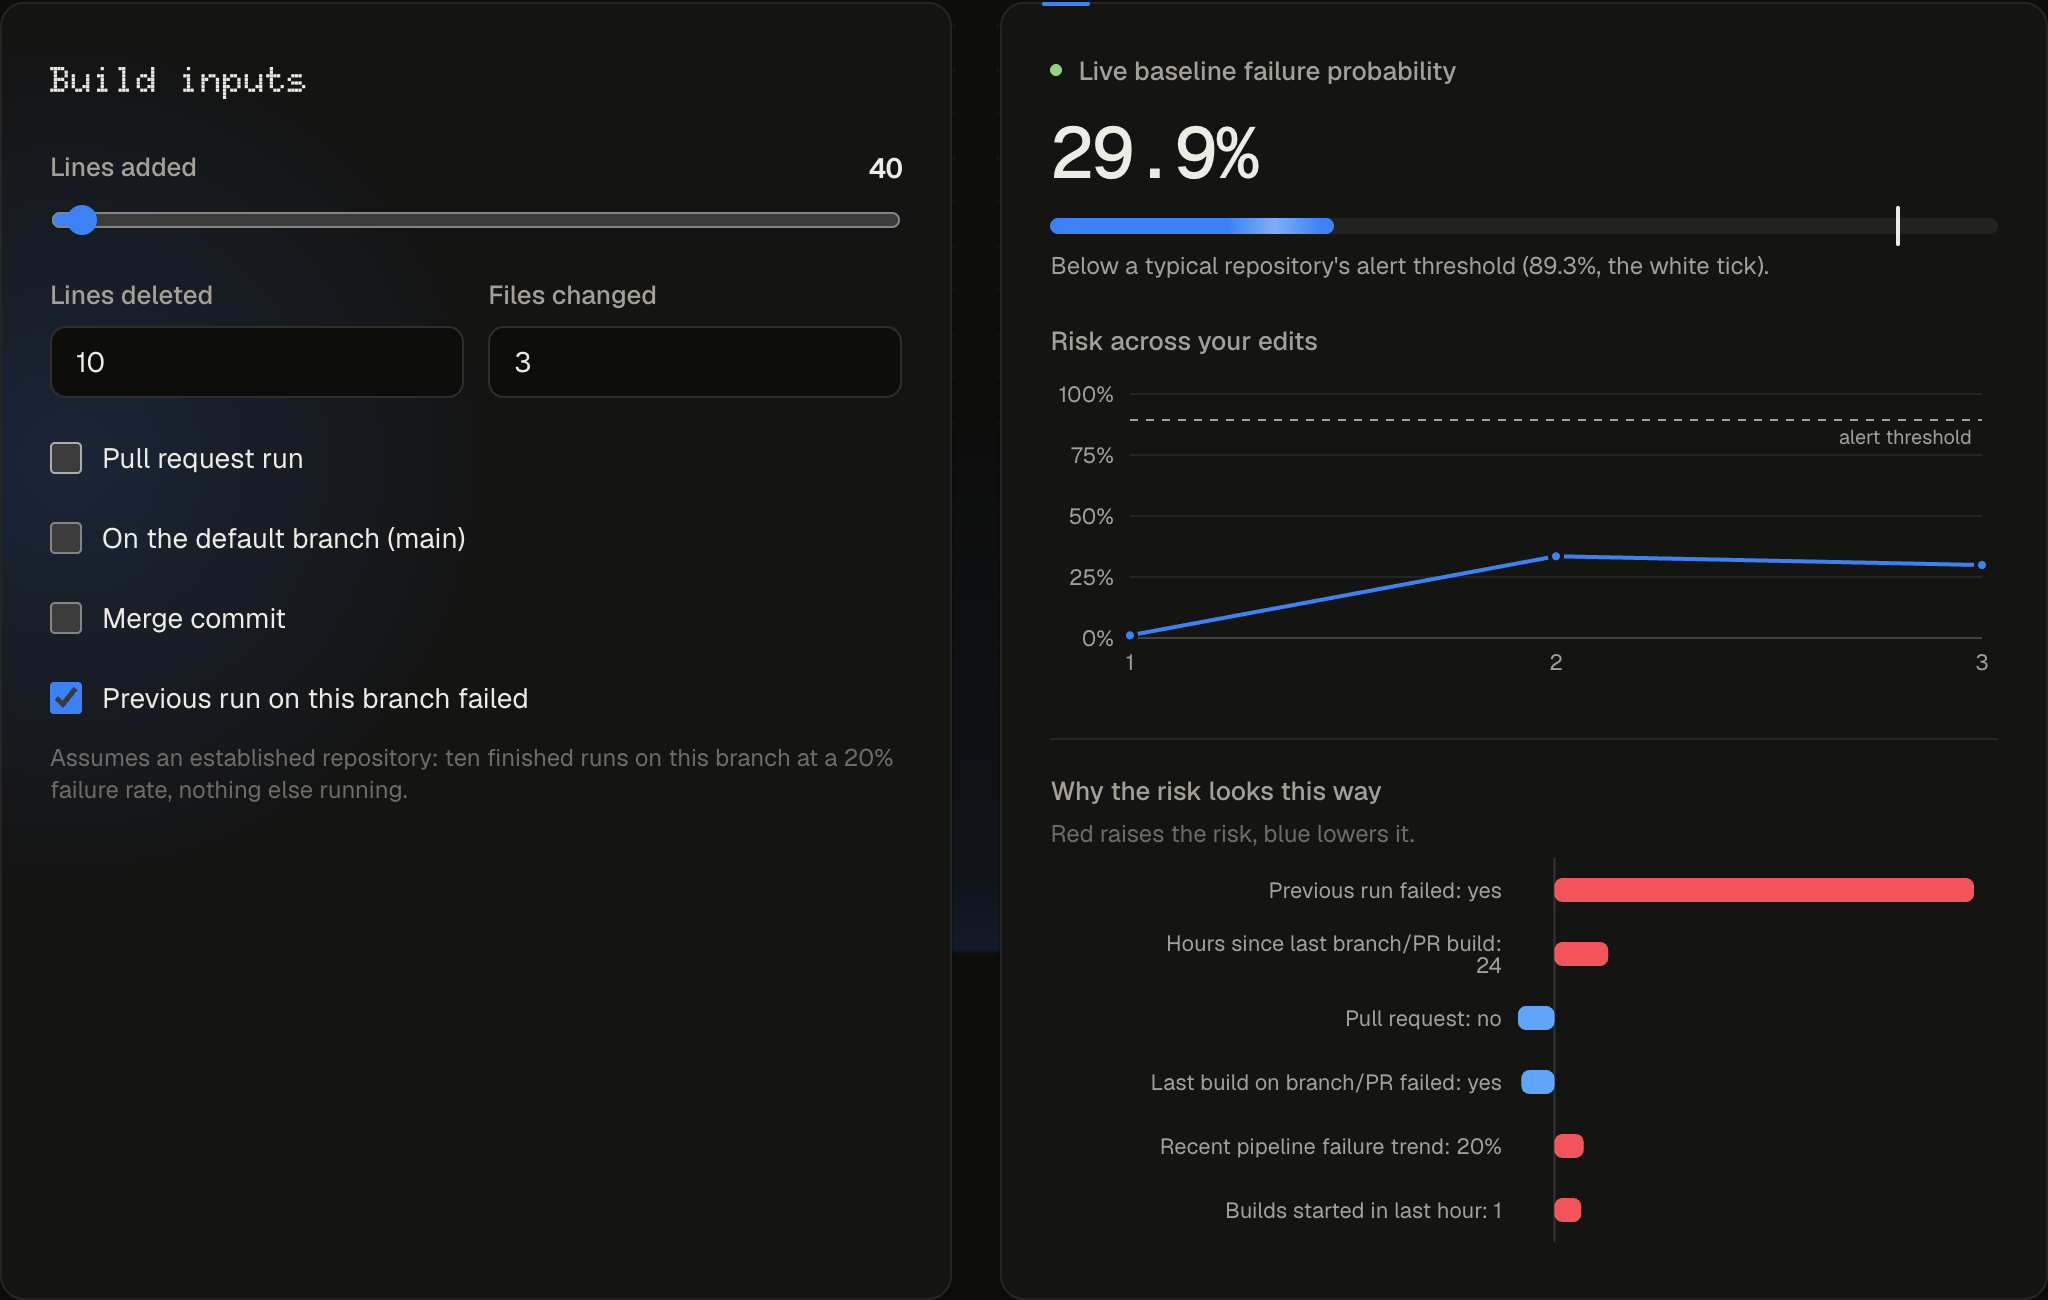
\includegraphics[width=0.9\textwidth]{what_if.png}
\caption{What-If page: whether the previous run of the same workflow failed dominates the explanation}
\label{fig:whatif}
\end{figure}

\section{Testing and Requirement Traceability}
\label{sec:testing}
The project has 84 automated tests, run by GitHub Actions on every pull request together with a production build of the dashboard. They cover:
\begin{itemize}
\item feature engineering, the availability registry and live-versus-training history equivalence;
\item the deployed model and the alert policy;
\item webhook signatures and the requested-to-completed flow, including late deliveries;
\item database migrations, the dashboard endpoints, PDF reports and the read-only demonstration mode.
\end{itemize}
Table~\ref{tab:trace} maps the requirements of Chapter~\ref{ch:srs} to their implementation.

{\renewcommand{\arraystretch}{1.3}
\begin{longtable}{|p{4.4cm}|p{6.2cm}|p{3.2cm}|}
\caption{Requirement-to-implementation traceability}\label{tab:trace}\\
\hline
\textbf{Requirement} & \textbf{Implementation} & \textbf{Verified by}\\ \hline
\endfirsthead
\hline
\textbf{Requirement} & \textbf{Implementation} & \textbf{Verified by}\\ \hline
\endhead
Data collection & TravisTorrent ingestion; GitHub Actions collector; signed webhooks & Webhook and signature tests\\ \hline
Preprocessing & Build collapsing, label rules, availability registry & Preprocessing and registry tests\\ \hline
Feature extraction & Finish-time-safe history, stream and in-flight context & Brute-force and equivalence tests\\ \hline
Failure prediction & \tierE\ model (LightGBM blend); RF, DT, SVM baselines & Model tests; reproduction check\\ \hline
Anomaly / bottleneck detection & Job timing vs.\ history; Isolation Forest & Bottleneck and anomaly tests\\ \hline
Root cause analysis & TF-IDF + k-means; rule-based log diagnosis & Clustering and log-analysis tests\\ \hline
Optimization suggestions & Category-to-suggestion rules; what-if simulation & Suggestion and simulator tests\\ \hline
Dashboard & React dashboard with charts, reports and alerts & Endpoint tests; production build\\ \hline
\end{longtable}}

\chapter{Results and Discussion}
\label{ch:results}

\section{Evaluation Protocol}
\label{sec:protocol}
All headline results use the following protocol, designed to match how a team would use the predictions.
\begin{itemize}
\item \textbf{Walk-forward folds.} Builds are sorted by trigger time and split into 10 equal chronological folds. Fold $k$ is tested after training on folds $1,\dots,k-1$, and the test folds are 6--10. On Travis~CI every design choice for \tierE\ was made on fold~6 alone; folds 7--10 were then scored once.
\item \textbf{Metric.} The primary metric is \emph{macro within-repository AUC}: the AUC computed within each repository that has both passes and failures in the test fold, averaged over repositories. 0.5 means random ranking and 1.0 perfect ranking. We also report \emph{recall@15\%}, the share of a repository's failures found when it reviews its riskiest 15\% of builds.
\item \textbf{Uncertainty.} Differences between models are paired by repository, and 95\% confidence intervals come from 1,000 bootstrap resamples of repositories~\cite{efron1993introduction}.
\item \textbf{Controls.} When training labels are randomly shuffled, the ranker drops to 0.48--0.50 within-repository AUC, as it should, which confirms that no label leaks into the features.
\item \textbf{Pre-registration.} Each GitHub Actions test followed a written protocol, fingerprinted (SHA-256) and committed before its data was collected~\cite{nosek2018preregistration}. Its decision rule was fixed in advance: \emph{confirms} if the mean gain over folds 6--10 is positive and at least 4 of 5 fold confidence intervals exclude zero; \emph{inconclusive} if the mean gain is positive otherwise; \emph{does not replicate} if it is not positive.
\end{itemize}

\section{How Much the Usual Evaluation Overstates Results}
\label{sec:leakage}
Table~\ref{tab:dev} and Fig~\ref{fig:modelcmp} compare the six classifiers in the way most studies do: a random 80/20 split of a 200,000-row sample. On this split, Random Forest, XGBoost and the stacking ensemble look strong (AUC 0.90--0.91, F1 about 0.73), while Decision Tree and SVM trail.

\begin{table}[H]
\centering
\caption{Development comparison of classifiers (random split; reference only)}
\label{tab:dev}
\begin{tabular}{|l|r|r|r|r|r|}
\hline
\textbf{Model} & \textbf{Accuracy} & \textbf{Precision} & \textbf{Recall} & \textbf{F1} & \textbf{AUC}\\ \hline
Stacking (RF + XGB + LGBM) & 0.899 & \textbf{0.831} & 0.653 & \textbf{0.731} & \textbf{0.912}\\ \hline
Random Forest & 0.889 & 0.749 & 0.714 & 0.731 & 0.908\\ \hline
XGBoost & 0.889 & 0.752 & 0.709 & 0.730 & 0.900\\ \hline
LightGBM & 0.877 & 0.699 & 0.729 & 0.714 & 0.898\\ \hline
Decision Tree & 0.769 & 0.469 & \textbf{0.741} & 0.575 & 0.825\\ \hline
SVM & 0.758 & 0.447 & 0.623 & 0.520 & 0.772\\ \hline
\end{tabular}
\end{table}

\begin{figure}[H]
\centering
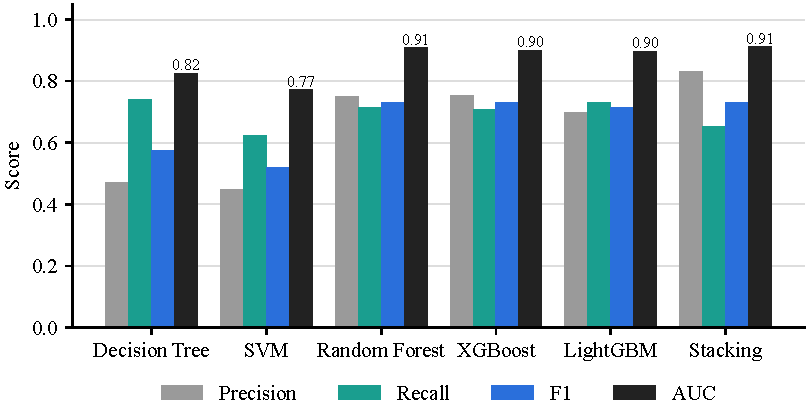
\includegraphics[width=0.95\textwidth]{model_comparison.pdf}
\caption{Development comparison of six classifiers on a random split (reference only)}
\label{fig:modelcmp}
\end{figure}

These numbers do \emph{not} describe real use. A random split lets a model learn each repository's future failure rate from builds that come later in time. Table~\ref{tab:leak} and Fig~\ref{fig:leakage} show the same task as the evaluation becomes progressively stricter:
\begin{itemize}
\item On a random split, adding fields from the build log lifts AUC from 0.690 to 0.896. Those fields are not available before a build runs, and the availability registry now blocks them.
\item Without leaky fields, the random-split AUC of 0.91 falls to 0.82 on a chronological split.
\item It falls to \textbf{0.63} when measured within each repository at the build level, which is how a team would experience it.
\end{itemize}
The rest of this chapter reports only this strict setting.

\begin{table}[H]
\centering
\caption{The same task under progressively stricter evaluation (Travis~CI)}
\label{tab:leak}
\begin{tabular}{|p{11cm}|r|}
\hline
\textbf{Setup} & \textbf{AUC}\\ \hline
Random split, 31 features including post-build log fields (leaky) & 0.896\\ \hline
Random split, 13 strict pre-build features & 0.690\\ \hline
Random split, 39 features with repository history (stacking) & 0.912\\ \hline
Chronological split, job level, pooled over repositories (Random Forest) & 0.821\\ \hline
Walk-forward, build level, \emph{within-repository} (\tierC\ Random Forest) & 0.628\\ \hline
Walk-forward, build level, \emph{within-repository} (\tierE, this project) & \textbf{0.698}\\ \hline
\end{tabular}
\end{table}

\begin{figure}[H]
\centering
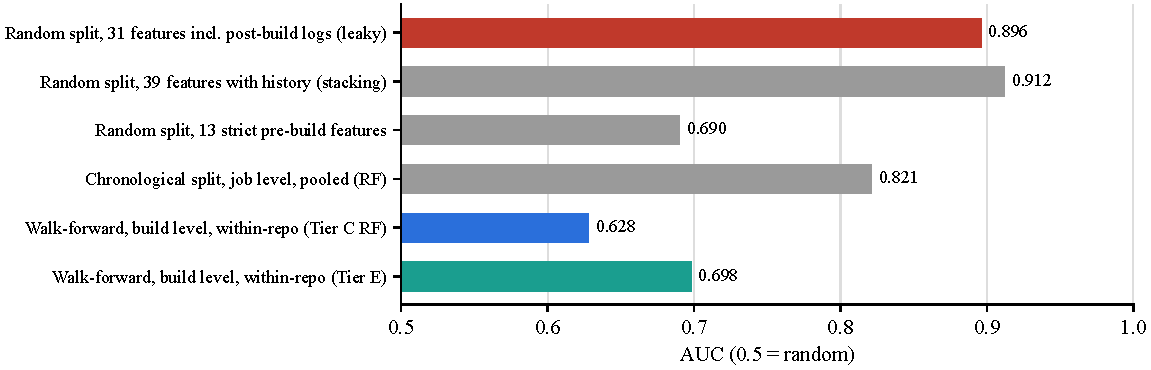
\includegraphics[width=0.95\textwidth]{leakage_ladder.pdf}
\caption{AUC under progressively stricter evaluation. Red: uses leaked post-build fields. Blue and teal: the strict protocol used for all results that follow.}
\label{fig:leakage}
\end{figure}

\section{Results on Travis CI}
\label{sec:travis}
Fig~\ref{fig:main} summarizes every evaluation. On Travis~CI, \tierE\ raises macro within-repository AUC from 0.628 to \textbf{0.698} (+0.070), and every confirmation fold's 95\% confidence interval is above zero. The per-fold gains are +0.068, +0.067, +0.070 and +0.074. Recall@15\% within each repository improves by +0.068.

\begin{figure}[H]
\centering
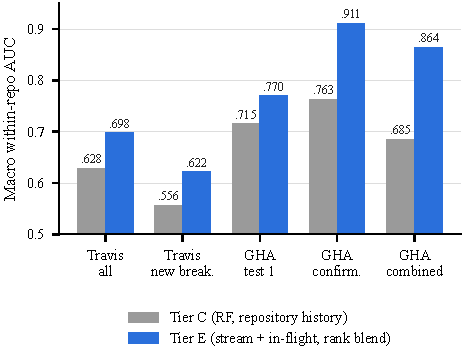
\includegraphics[width=0.78\textwidth]{main_results.pdf}
\caption{Macro within-repository AUC of \tierC\ (Random Forest with repository history) and \tierE\ across all evaluations (test folds; outcomes known as soon as builds finish)}
\label{fig:main}
\end{figure}

\minorhead{Robustness to reporting delays}
Table~\ref{tab:travis} repeats the evaluation with outcomes withheld for an extra 1 or 6 hours. Unlike a pure ``it failed last time'' effect, the gain \emph{grows} as outcomes are withheld longer (Fig~\ref{fig:buffer}). The in-flight features, such as whether the previous build is still running, stay informative when recent outcomes are not yet known.

\begin{table}[H]
\centering
\caption{Travis~CI results by finish buffer (folds 7--10). Every fold's 95\% CI for the gain is above zero.}
\label{tab:travis}
\begin{tabular}{|c|r|r|r|}
\hline
\textbf{Finish buffer} & \textbf{\tierC\ Random Forest} & \textbf{\tierE} & \textbf{Gain}\\ \hline
0 h & 0.628 & \textbf{0.698} & +0.070\\ \hline
1 h & 0.600 & \textbf{0.681} & +0.081\\ \hline
6 h & 0.585 & \textbf{0.672} & +0.087\\ \hline
\end{tabular}
\end{table}

\begin{figure}[H]
\centering
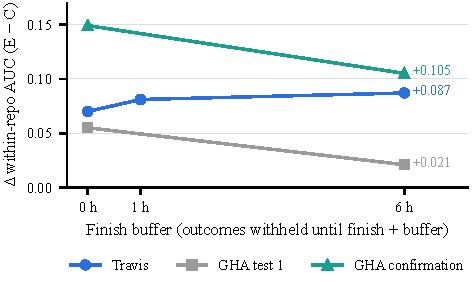
\includegraphics[width=0.72\textwidth]{finish_buffer.pdf}
\caption{Gain of \tierE\ over \tierC\ as outcomes are withheld longer}
\label{fig:buffer}
\end{figure}

\minorhead{What drives the gain}
Table~\ref{tab:attr} separates the ingredients.
\begin{itemize}
\item The learning-to-rank objective is the largest single lever on Travis~CI: it is worth +0.031 on \tierC\ features alone.
\item Stream and in-flight features add about +0.03 more.
\item Build-matrix size, the number of jobs, adds only about 0.003, so the deployed variant omits it.
\end{itemize}
The ranker trades overall (pooled) AUC for within-repository ordering. Teams that need a pooled ranking across repositories should use the binary \tierE\ model, which beats \tierC\ on both measures.

\begin{table}[H]
\centering
\caption{Attribution of the \tierE\ gain on Travis~CI (folds 7--10)}
\label{tab:attr}
\begin{tabular}{|l|r|r|}
\hline
\textbf{Variant} & \textbf{Within-repo AUC} & \textbf{Pooled AUC}\\ \hline
\tierC, Random Forest & 0.628 & 0.856\\ \hline
\tierC, binary LightGBM & 0.633 & --\\ \hline
\tierC, LightGBM ranker & 0.664 & --\\ \hline
\tierE, binary LightGBM & 0.652 & \textbf{0.881}\\ \hline
\tierE, LightGBM ranker & 0.696 & --\\ \hline
\tierE, blend & \textbf{0.698} & 0.828\\ \hline
\tierE, blend without job counts & 0.695 & 0.826\\ \hline
\end{tabular}
\end{table}

\section{New Breakages}
\label{sec:newbreak}
Much of the signal comes from branches or pull requests that are already failing: 55\% of failures occur on streams whose last known outcome was a failure. To check that the model does more than repeat the last outcome, the saved predictions were rescored on \emph{new breakages}, builds whose previous build on the same stream passed. These are 25\% of failures, and such builds fail only 6.6\% of the time.
\begin{itemize}
\item On new breakages, the repository's recent failure rate is at chance (0.504) and \tierC\ scores 0.556.
\item \tierE\ scores \textbf{0.622}, a gain of +0.066, as large as on all builds, with every fold's interval above zero.
\item With a 15\% review budget, \tierE\ catches 30\% of new breakages (lift 1.78$\times$) against 24\% for \tierC.
\end{itemize}
The honest headline for \emph{fresh} breakages is therefore about 0.62, not 0.70. This analysis was carried out after the main results (post hoc).

\section{Pre-Registered Tests on GitHub Actions}
\label{sec:gha}
The frozen recipe was tested on GitHub Actions, a different CI platform, without any changes.

\minorhead{Test 1 (30 repositories): inconclusive}
\tierE\ scored 0.770 against 0.715 (+0.055) and was ahead in all five folds. However, only 3 of 5 fold intervals excluded zero, and the rule required 4, so the pre-registered verdict is \emph{inconclusive} (Table~\ref{tab:gha1}). Recall@15\% was 0.48 against 0.37.

\begin{table}[H]
\centering
\caption{First GitHub Actions test (30 repositories, folds 6--10)}
\label{tab:gha1}
\begin{tabular}{|l|r|r|r|c|}
\hline
\textbf{Setting} & \textbf{\tierC} & \textbf{\tierE} & \textbf{Gain} & \textbf{Folds clearly ahead}\\ \hline
All runs (primary) & 0.715 & \textbf{0.770} & +0.055 & 3/5\\ \hline
Label-validity check & 0.703 & 0.754 & +0.051 & 3/5\\ \hline
New breakages & 0.645 & 0.695 & +0.050 & 0/5\\ \hline
All runs, 6 h buffer & 0.698 & 0.718 & +0.021 & 0/5\\ \hline
\end{tabular}
\end{table}

\minorhead{Confirmation (30 new repositories): confirms}
A second protocol was fixed before collecting data from 30 repositories never used before. Here \tierE\ scored \textbf{0.911} against 0.763 (+0.149). All five fold intervals exclude zero, and the smallest lower bound is +0.090 (Fig~\ref{fig:folds}, Table~\ref{tab:confirm}). Recall@15\% rose from 0.31 to 0.43, and \tierE\ beat \tierC\ in all 24 test repositories. A secondary analysis on both datasets together (60 repositories) gave +0.179, again 5 of 5 folds.

\begin{figure}[H]
\centering
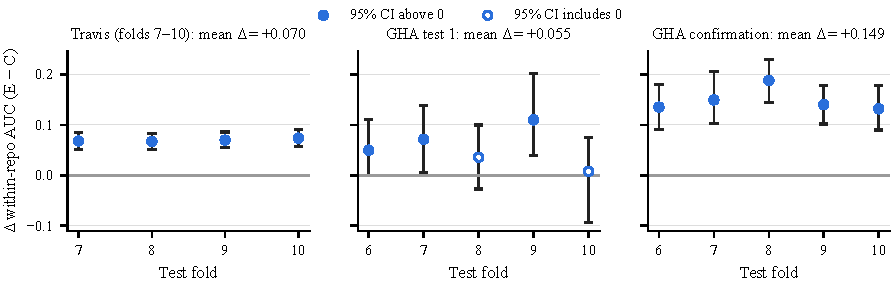
\includegraphics[width=\textwidth]{fold_deltas.pdf}
\caption{Per-fold gain of \tierE\ over \tierC\ with 95\% confidence intervals. Filled markers: the interval excludes zero.}
\label{fig:folds}
\end{figure}

\begin{table}[H]
\centering
\caption{GitHub Actions confirmation test (30 new repositories, folds 6--10)}
\label{tab:confirm}
\begin{tabular}{|l|r|r|r|c|}
\hline
\textbf{Setting} & \textbf{\tierC} & \textbf{\tierE} & \textbf{Gain} & \textbf{Folds clearly ahead}\\ \hline
All runs (primary) & 0.763 & \textbf{0.911} & +0.149 & 5/5\\ \hline
Label-validity check & 0.765 & 0.911 & +0.147 & 5/5\\ \hline
New breakages & 0.642 & 0.683 & +0.041 & 2/5\\ \hline
All runs, 6 h buffer & 0.741 & 0.846 & +0.105 & 5/5\\ \hline
New breakages, 6 h buffer & 0.637 & 0.634 & $-$0.004 & 0/5\\ \hline
Combined, 60 repositories & 0.685 & 0.864 & +0.179 & 5/5\\ \hline
\end{tabular}
\end{table}

\minorhead{Is it only ``it failed last time''?}
The confirmation gain is almost three times the first test's, and failures were three times as common. We therefore checked a naive rule that predicts failure when the stream's previous finished run failed. It scores only about 0.72, below \tierC\ (Fig~\ref{fig:persist}), and the gain per repository is unrelated to the repository's failure rate (correlation 0.03). This check was exploratory.

\begin{figure}[H]
\centering
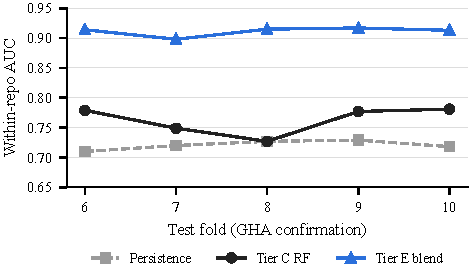
\includegraphics[width=0.75\textwidth]{persistence.pdf}
\caption{Confirmation test: \tierE\ against \tierC\ and a naive persistence rule}
\label{fig:persist}
\end{figure}

\minorhead{Discussion}
On GitHub Actions, the stream and in-flight features carry the gain; the ranking objective alone adds only +0.010 (test~1) and +0.042 (confirmation). Most runs finish within an hour, so the very recent outcome of the same stream is the key signal. Withholding it for 6 hours removes most of the gain on new breakages. The size of the gain varies by project (+0.055 to +0.149), but its direction is consistent across Travis~CI and both GitHub Actions tests.

\section{Deployed Model and Alert Policy}
\label{sec:alerts}
The deployed model was trained on folds 1--9 of the 146,556 GitHub Actions runs. Table~\ref{tab:holdout} shows its results on the newest 10\%. To estimate how it performs on a repository it has never seen, the holdout was rescored with all workflow identities hidden; it still reaches 0.893.

\begin{table}[H]
\centering
\caption{Deployed model on its holdout (newest 10\% of GitHub Actions runs, 20 repositories)}
\label{tab:holdout}
\begin{tabular}{|l|r|}
\hline
\textbf{Measure} & \textbf{Value}\\ \hline
Within-repository AUC & 0.913\\ \hline
Within-repository AUC, repository never seen & 0.893\\ \hline
Within-repository recall at a 15\% review budget & 43.3\%\\ \hline
Pooled AUC & 0.936\\ \hline
Failure rate of the holdout & 36.3\%\\ \hline
\end{tabular}
\end{table}

\minorhead{Alert policy}
A single global threshold set to flag 15\% of the holdout sits at 0.94, because that holdout fails often. It flags between 3\% and 51\% of a repository's runs. The per-repository budget instead flags each repository's riskiest 15\% of recent runs (Section~\ref{sec:deployed}). Replayed in time order on the holdout, each repository flags 11--22\% of its runs, and the share of a repository's failures caught rises from 34\% to 41\%, close to the 43\% measured in hindsight (Table~\ref{tab:alert}, Fig~\ref{fig:alert}). Pooled precision is lower only because the global threshold spends almost all its alerts on the repositories that fail most.

\begin{table}[H]
\centering
\caption{Alert policies compared on the deployed model's holdout}
\label{tab:alert}
\begin{tabular}{|l|r|r|}
\hline
\textbf{Measure} & \textbf{Global threshold (0.94)} & \textbf{Per-repository budget}\\ \hline
Runs flagged per repository & 3--51\% & 11--22\%\\ \hline
Failures caught per repository (mean) & 34\% & \textbf{41\%}\\ \hline
Share of alerts that were failures & 0.97 & 0.80\\ \hline
\end{tabular}
\end{table}

\begin{figure}[H]
\centering
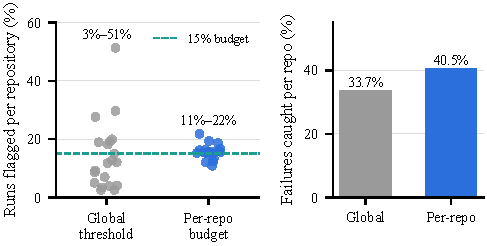
\includegraphics[width=0.75\textwidth]{alert_policy.pdf}
\caption{Global threshold vs.\ per-repository alert budget: share of each repository's runs flagged (left) and failures caught (right)}
\label{fig:alert}
\end{figure}

\minorhead{Public demonstration}
In the public demonstration, the 450 replayed runs are scored with the history the system builds up live, starting empty. Within-repository AUCs are 0.80 (freeCodeCamp), 0.95 (bootstrap) and 0.74 (yt-dlp), close to the research evaluation of the same runs (0.78, 0.97 and 0.79). The model-evidence panel of the dashboard (Fig~\ref{fig:dash_models}) presents these research results alongside the deployed model's holdout statistics.

\begin{figure}[H]
\centering
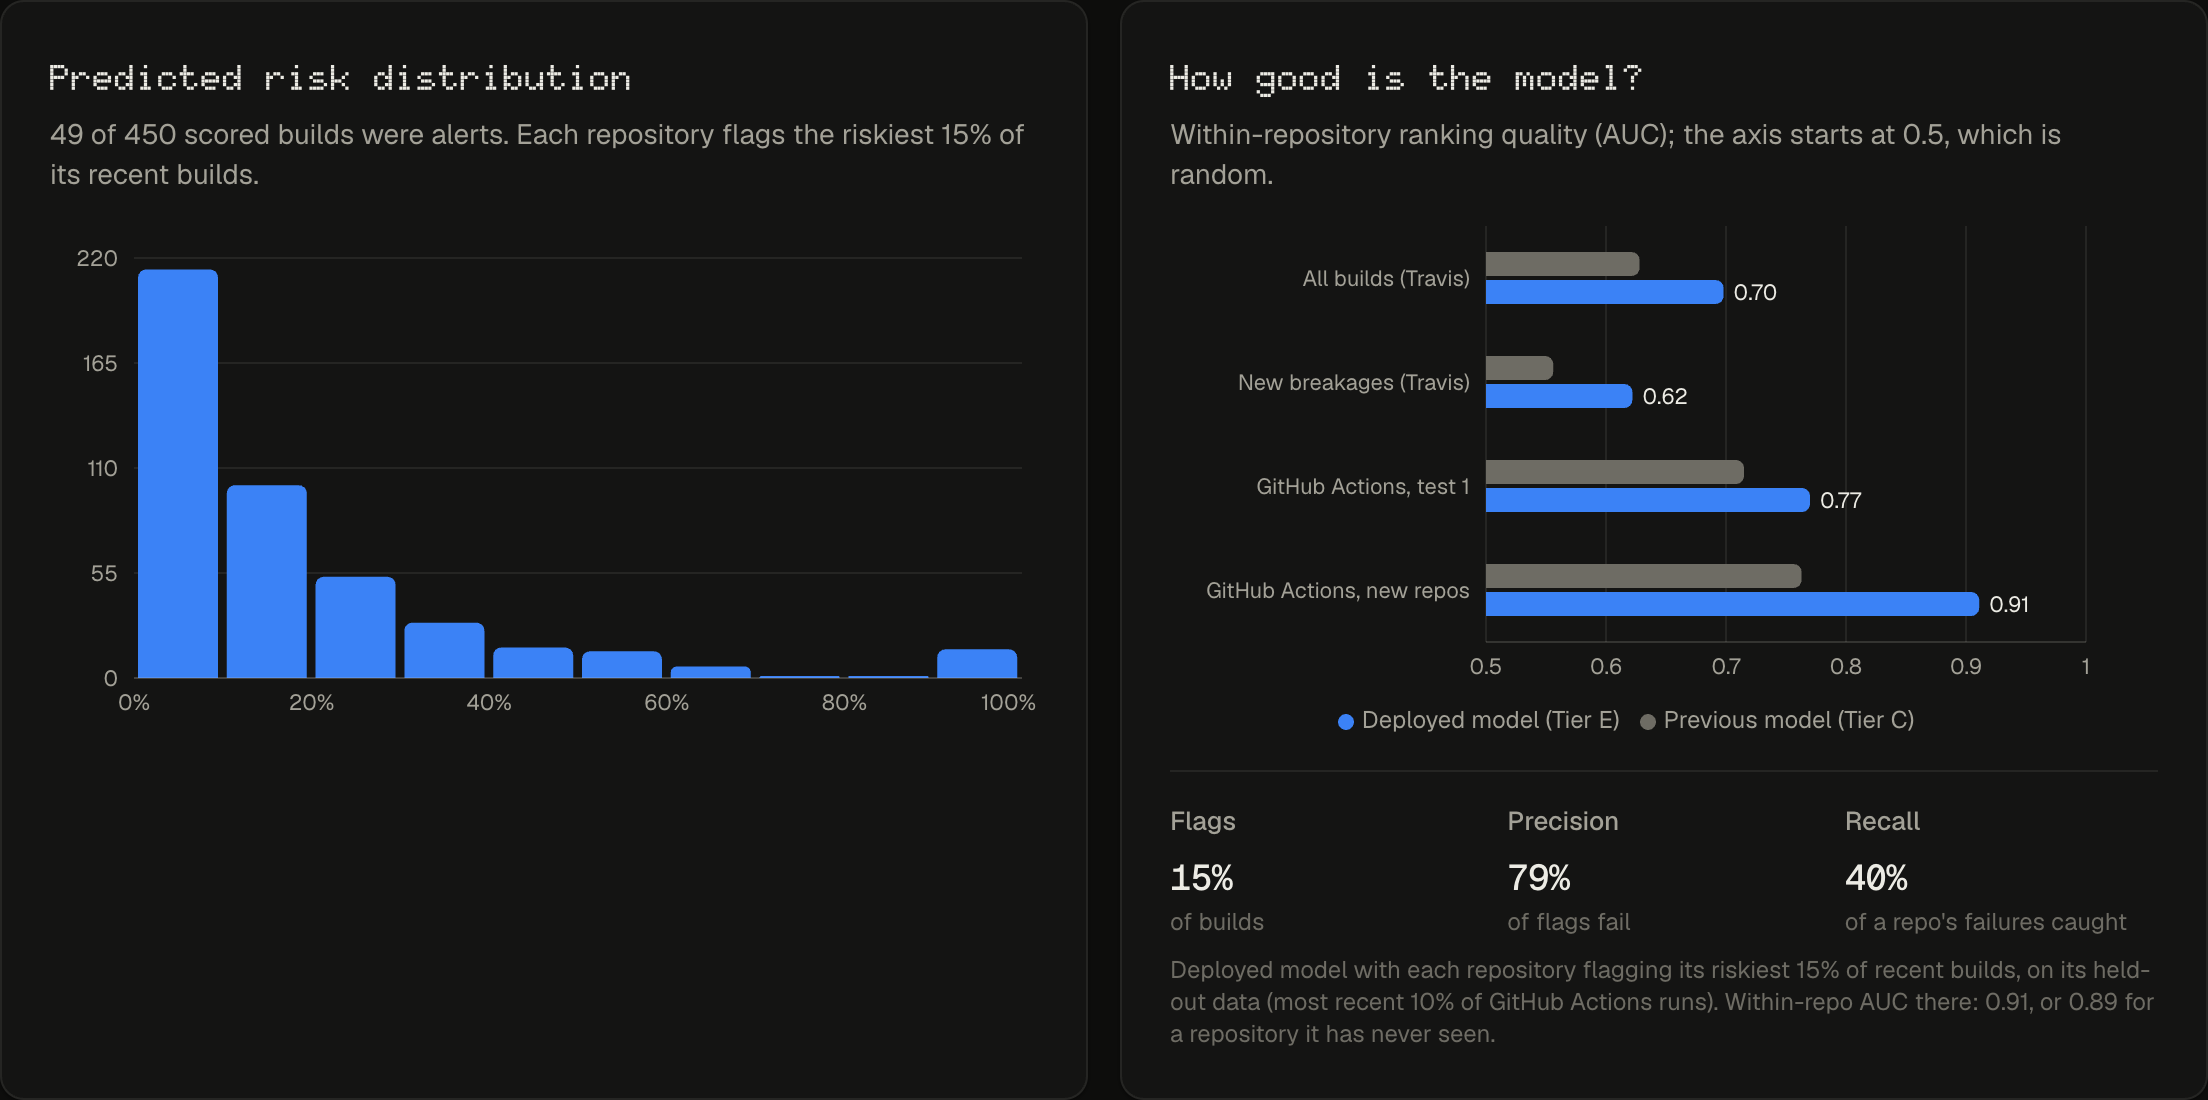
\includegraphics[width=\textwidth]{dashboard_models.png}
\caption{Dashboard: risk distribution of the 450 demonstration runs (49 alerts under the per-repository budget) and the model-evidence panel}
\label{fig:dash_models}
\end{figure}

\section{Negative Results}
\label{sec:negative}
\begin{itemize}
\item \textbf{Repository-level streaks hurt.} Adding repository-level failure streaks and time gaps to \tierC\ \emph{reduced} within-repository AUC by 0.019, significantly in 4 of 5 folds. Streaks that mix all of a repository's branches are noise; per-stream history is the version of this idea that helps.
\item \textbf{Anomaly flag.} Builds flagged as anomalous by Isolation Forest did not fail more often, so the flag is kept as a diagnostic rather than presented as a risk signal.
\end{itemize}

\section{Threats to Validity}
\label{sec:threats}
\begin{itemize}
\item \textbf{Post-hoc analyses.} The new-breakage analysis and the persistence check were carried out after the main results. On Travis~CI fold~6 was used for development, so only folds 7--10 are confirmatory.
\item \textbf{Approximate finish times.} Finish times on Travis~CI are derived from job durations, with a fallback for missing ones.
\item \textbf{Lost runs.} In the confirmation data, 4.6\% of runs were lost to unfetchable fork commits, and these runs failed more often (38.5\% vs.\ 28.2\%).
\item \textbf{Selection.} Repositories come from popular open-source projects. Capping each repository at 4,000 runs left six of the busiest projects in training folds only.
\item \textbf{What the metric measures.} Within-repository AUC measures ranking, not calibrated probability. Recall at a 15\% budget assumes that teams review a fixed share of builds.
\end{itemize}

\chapter{Conclusion and Future Work}
\label{ch:conclusion}

\section{Conclusion}
CI/CD has made the integration, testing and deployment of code largely automatic. Yet frequent build failures, long execution times, dependency issues and manual debugging remain challenges, and current CI/CD systems concentrate on automation and monitoring rather than failure prediction and optimization.

This project designed, built and evaluated an AI-based system that predicts CI/CD build failures before a build runs, detects bottlenecks, groups and diagnoses failures, and presents the results on a dashboard. The main conclusions are:
\begin{itemize}
\item \textbf{Evaluation matters as much as the model.} The same kind of classifier scores 0.91 AUC on a random split but only 0.63 under a protocol that matches real use. That protocol uses only information available at trigger time, counts a past build only once it has finished, evaluates chronologically, and measures ranking within each repository. Results that skip these steps should not be trusted.
\item \textbf{Stream-aware ranking works.} Adding the history of the build's own branch or pull request, the state of builds still running, and a learning-to-rank objective improved within-repository AUC on Travis~CI from 0.628 to 0.698. It also improved from 0.556 to 0.622 on new breakages, where the last outcome gives no clue.
\item \textbf{The result carries over.} Tested on GitHub Actions under protocols fixed in advance, the gain was positive in every fold. The first test was inconclusive under its strict rule (3 of 5 folds); a confirmation on 30 new repositories met the rule in all five folds (0.911 vs.\ 0.763).
\item \textbf{The system is usable.} The deployed service scores GitHub Actions runs automatically and explains each prediction. Each repository reviews its riskiest 15\% of runs, which catches about 41\% of its failures. A read-only public demonstration shows the system on real, out-of-sample runs.
\end{itemize}

\minorhead{Objectives achieved}
\begin{enumerate}
\item \textit{Predict build failures from historical data.} Achieved, with a leakage-safe protocol and pre-registered external confirmation (Sections~\ref{sec:travis}--\ref{sec:gha}).
\item \textit{Detect bottlenecks and abnormal execution.} Achieved: job durations are compared with their own history to flag slow and stalled jobs, and Isolation Forest flags unusual inputs (Section~\ref{sec:aux}).
\item \textit{Automated root cause analysis and suggestions on a dashboard.} Achieved: failure logs are clustered and diagnosed, each category maps to a suggestion, and everything is presented on the dashboard (Sections~\ref{sec:aux} and~\ref{sec:dashboard}).
\end{enumerate}

\section{Future Work}
\begin{itemize}
\item \textbf{Forward-looking test.} A test of the frozen deployed system has been pre-registered. It will score October~2026 runs from the 60 repositories, collected from 28~November~2026, with the model and alert rule fixed by their SHA-256 fingerprints. It counts as holding up if the model clearly beats a ``last run failed'' baseline and reaches at least 0.80 within-repository AUC.
\item \textbf{Earlier warning for first failures.} Gains on new breakages are smaller and vanish when outcomes are delayed. Richer change information, such as which files and tests a change touches, may help.
\item \textbf{More CI platforms.} Collect and evaluate data from GitLab CI/CD and Jenkins, beyond the existing Jenkins endpoint.
\item \textbf{Large-scale deployment.} Run the service on Kubernetes with a production database, and add per-team configuration of the review budget.
\item \textbf{Deeper log analysis.} Use natural language processing models for log understanding and root cause identification, and explore automated self-repair for common failure types.
\item \textbf{Calibrated probabilities per repository}, so that a predicted risk can be read as a real chance of failure.
\end{itemize}

These enhancements would further improve the CI/CD optimization system in effectiveness and reach.

\chapter{References}
\label{ch:references}
\renewcommand{\bibname}{}
\begingroup
\renewcommand{\chapter}[2]{}% the chapter heading above replaces thebibliography's own
\small
\begin{thebibliography}{99}
\setlength{\itemsep}{3pt}

\bibitem{zhang2022buildsheriff} C. Zhang, B. Chen, X. Peng, and W. Zhao, ``BuildSheriff: Change-aware test failure triage for continuous integration builds,'' in \emph{Proc. 44th Int. Conf. Software Engineering (ICSE)}, 2022. [Online]. Available: \url{https://chenbihuan.github.io/paper/icse22-zhang-buildsheriff.pdf}

\bibitem{saidani2020predicting} I. Saidani, A. Ouni, M. Chouchen, and M. W. Mkaouer, ``Predicting continuous integration build failures using evolutionary search,'' \emph{Information and Software Technology}, 2020. [Online]. Available: \url{https://ouniali.github.io/papers/IST2020-saidani.pdf}

\bibitem{barrak2021why} A. Barrak, E. E. Eghan, B. Adams, and F. Khomh, ``Why do builds fail? A conceptual replication study,'' \emph{Journal of Systems and Software}, 2021. [Online]. Available: \url{https://www.sciencedirect.com/science/article/abs/pii/S0164121221000364}

\bibitem{rausch2017empirical} T. Rausch, W. Hummer, P. Leitner, and S. Schulte, ``An empirical analysis of build failures in the continuous integration workflows of Java-based open-source software,'' in \emph{Proc. 14th Int. Conf. Mining Software Repositories (MSR)}, 2017, pp.~345--355. [Online]. Available: \url{https://ieeexplore.ieee.org/document/7962384}

\bibitem{durieux2020empirical} T. Durieux, C. Le Goues, M. Hilton, and R. Abreu, ``Empirical study of restarted and flaky builds on Travis CI,'' in \emph{Proc. 17th Int. Conf. Mining Software Repositories (MSR)}, 2020. [Online]. Available: \url{https://2020.msrconf.org/details/msr-2020-papers/21}

\bibitem{ghaleb2019empirical} T. A. Ghaleb, D. A. da Costa, and Y. Zou, ``An empirical study of the long duration of continuous integration builds,'' \emph{Empirical Software Engineering}, 2019. [Online]. Available: \url{https://link.springer.com/article/10.1007/s10664-019-09695-9}

\bibitem{saidani2022improving} I. Saidani, A. Ouni, and M. W. Mkaouer, ``Improving the prediction of continuous integration build failures using deep learning,'' \emph{Automated Software Engineering}, 2022. [Online]. Available: \url{https://www.researchgate.net/publication/357990835}

\bibitem{farihane2025ci} R. Farihane, ``CI/CD pipeline optimization using AI: A systematic mapping study,'' \emph{MDPI Proceedings}, 2025.

\bibitem{kumar2025optimizing} R. Kumar, D. N. D. Kollipara, A. H. Mohammed, S. Kumar, F. B. Mohammed, and A. Kumar, ``Optimizing CI/CD pipelines with AI-driven build failure prediction: An empirical study on machine learning models for early failure detection,'' 2025.

\bibitem{hong2024practitioners} Y. Hong, C. Tantithamthavorn, J. Pasuksmit, P. Thongtanunam, A. Friedman, X. Zhao, and A. Krasikov, ``Practitioners' challenges and perceptions of CI build failure predictions at Atlassian,'' arXiv preprint arXiv:2402.09651, 2024.

\bibitem{hilton2016usage} M. Hilton, T. Tunnell, K. Huang, D. Marinov, and D. Dig, ``Usage, costs, and benefits of continuous integration in open-source projects,'' in \emph{Proc. 31st IEEE/ACM Int. Conf. Automated Software Engineering (ASE)}, 2016, pp.~426--437.

\bibitem{beller2017travistorrent} M. Beller, G. Gousios, and A. Zaidman, ``TravisTorrent: Synthesizing Travis CI and GitHub for full-stack research on continuous integration,'' in \emph{Proc. 14th Int. Conf. Mining Software Repositories (MSR)}, 2017, pp.~447--450.

\bibitem{hassan2017change} F. Hassan and X. Wang, ``Change-aware build prediction model for stall avoidance in continuous integration,'' in \emph{Proc. ACM/IEEE Int. Symp. Empirical Software Engineering and Measurement (ESEM)}, 2017, pp.~157--162.

\bibitem{ni2017cost} A. Ni and M. Li, ``Cost-effective build outcome prediction using cascaded classifiers,'' in \emph{Proc. 14th Int. Conf. Mining Software Repositories (MSR)}, 2017, pp.~455--458.

\bibitem{xia2017could} J. Xia and Y. Li, ``Could we predict the result of a continuous integration build? An empirical study,'' in \emph{Proc. IEEE Int. Conf. Software Quality, Reliability and Security Companion (QRS-C)}, 2017, pp.~311--315.

\bibitem{chen2020buildfast} B. Chen, L. Chen, C. Zhang, and X. Peng, ``BuildFast: History-aware build outcome prediction for fast feedback and reduced cost in continuous integration,'' in \emph{Proc. 35th IEEE/ACM Int. Conf. Automated Software Engineering (ASE)}, 2020, pp.~42--53.

\bibitem{jin2020cost} X. Jin and F. Servant, ``A cost-efficient approach to building in continuous integration,'' in \emph{Proc. 42nd ACM/IEEE Int. Conf. Software Engineering (ICSE)}, 2020, pp.~13--25.

\bibitem{gallaba2018noise} K. Gallaba, C. Macho, M. Pinzger, and S. McIntosh, ``Noise and heterogeneity in historical build data: An empirical study of Travis CI,'' in \emph{Proc. 33rd ACM/IEEE Int. Conf. Automated Software Engineering (ASE)}, 2018, pp.~87--97.

\bibitem{durieux2019analysis} T. Durieux, R. Abreu, M. Monperrus, T. F. Bissyandé, and L. Cruz, ``An analysis of 35+ million jobs of Travis CI,'' in \emph{Proc. IEEE Int. Conf. Software Maintenance and Evolution (ICSME)}, 2019, pp.~291--295.

\bibitem{kaufman2012leakage} S. Kaufman, S. Rosset, C. Perlich, and O. Stitelman, ``Leakage in data mining: Formulation, detection, and avoidance,'' \emph{ACM Trans. Knowledge Discovery from Data}, vol.~6, no.~4, 2012.

\bibitem{bergmeir2012use} C. Bergmeir and J. M. Benítez, ``On the use of cross-validation for time series predictor evaluation,'' \emph{Information Sciences}, vol.~191, pp.~192--213, 2012.

\bibitem{nosek2018preregistration} B. A. Nosek, C. R. Ebersole, A. C. DeHaven, and D. T. Mellor, ``The preregistration revolution,'' \emph{Proc. National Academy of Sciences}, vol.~115, no.~11, pp.~2600--2606, 2018.

\bibitem{breiman2001random} L. Breiman, ``Random forests,'' \emph{Machine Learning}, vol.~45, no.~1, pp.~5--32, 2001.

\bibitem{quinlan1986induction} J. R. Quinlan, ``Induction of decision trees,'' \emph{Machine Learning}, vol.~1, no.~1, pp.~81--106, 1986.

\bibitem{cortes1995support} C. Cortes and V. Vapnik, ``Support-vector networks,'' \emph{Machine Learning}, vol.~20, no.~3, pp.~273--297, 1995.

\bibitem{chen2016xgboost} T. Chen and C. Guestrin, ``XGBoost: A scalable tree boosting system,'' in \emph{Proc. 22nd ACM SIGKDD Int. Conf. Knowledge Discovery and Data Mining}, 2016, pp.~785--794.

\bibitem{ke2017lightgbm} G. Ke, Q. Meng, T. Finley, T. Wang, W. Chen, W. Ma, Q. Ye, and T.-Y. Liu, ``LightGBM: A highly efficient gradient boosting decision tree,'' in \emph{Advances in Neural Information Processing Systems (NeurIPS)}, vol.~30, 2017.

\bibitem{bruch2021alternative} S. Bruch, ``An alternative cross entropy loss for learning-to-rank,'' in \emph{Proc. Web Conference (WWW)}, 2021, pp.~118--126.

\bibitem{platt1999probabilistic} J. C. Platt, ``Probabilistic outputs for support vector machines and comparisons to regularized likelihood methods,'' in \emph{Advances in Large Margin Classifiers}. MIT Press, 1999, pp.~61--74.

\bibitem{lundberg2017unified} S. M. Lundberg and S.-I. Lee, ``A unified approach to interpreting model predictions,'' in \emph{Advances in Neural Information Processing Systems (NeurIPS)}, vol.~30, 2017.

\bibitem{liu2008isolation} F. T. Liu, K. M. Ting, and Z.-H. Zhou, ``Isolation forest,'' in \emph{Proc. 8th IEEE Int. Conf. Data Mining (ICDM)}, 2008, pp.~413--422.

\bibitem{pedregosa2011scikit} F. Pedregosa \emph{et al.}, ``Scikit-learn: Machine learning in Python,'' \emph{Journal of Machine Learning Research}, vol.~12, pp.~2825--2830, 2011.

\bibitem{salton1988term} G. Salton and C. Buckley, ``Term-weighting approaches in automatic text retrieval,'' \emph{Information Processing \& Management}, vol.~24, no.~5, pp.~513--523, 1988.

\bibitem{lloyd1982least} S. P. Lloyd, ``Least squares quantization in PCM,'' \emph{IEEE Trans. Information Theory}, vol.~28, no.~2, pp.~129--137, 1982.

\bibitem{efron1993introduction} B. Efron and R. J. Tibshirani, \emph{An Introduction to the Bootstrap}. Chapman \& Hall, 1993.

\end{thebibliography}
\endgroup

\vspace{6pt}
\noindent\textbf{Project resources.} Source code, protocols and results: \url{https://github.com/yasaswinipakam/cicd-ai-optimizer}. Read-only demonstration: \url{https://cicd-ai-optimizer.onrender.com}.

\end{document}
